%!TeX spellcheck = en-GB

%Basics
\documentclass[aps, prb, a4paper, english, 12pt, onecolumn, longbibliography, amsmath, amssymb, colorinlistoftodos, floatfix]{revtex4-1}
\usepackage[utf8]{inputenc}
\usepackage{babel}

%Symbols and scientifics
\usepackage{amsmath, amsfonts, amssymb, bm}
\usepackage{physics}
\usepackage{mathtools}
\usepackage{siunitx}
\sisetup{
	per-mode = power ,
	round-mode = figures ,
	round-precision = 3 ,
	scientific-notation = false ,
	output-decimal-marker = {.} ,
	exponent-product = \times ,
	separate-uncertainty = true ,
	uncertainty-separator = \ ,
	output-product = \cdot ,
	quotient-mode = fraction ,
	range-phrase = - ,
	range-units =  single ,
	inter-unit-product = \ensuremath{{\cdot{}}} ,
	number-unit-product = \ ,
	multi-part-units = single ,
	alsoload = synchem ,
}
\DeclareSIUnit\atm{atm}

%Appendix, TOC and Bibliography
\usepackage{appendix}
\renewcommand\appendixtocname{Appendices}
%\usepackage[nottoc]{tocbibind}
\usepackage[lastpage,user]{zref}

%Figures
\usepackage[svgnames]{xcolor} % Required to specify font color
\usepackage{float}
\usepackage{graphicx}
\usepackage{subcaption}
\usepackage{caption}
\usepackage{wrapfig}
\usepackage[a4paper, centering, rmargin=2.5cm, tmargin=2.5cm, lmargin=2.5cm, bmargin=2.5cm]{geometry}
\usepackage{etoolbox}
\usepackage{verbatim}
\usepackage[space]{grffile}
\usepackage[final]{pdfpages}
\usepackage{array}
\usepackage{multirow}
\usepackage{dcolumn}
%\usepackage{animate}
\usepackage{fontawesome}
\usepackage[european]{circuitikz}
\usepackage{pgfplots}
\pgfplotsset{width=10cm}
\usepgfplotslibrary{external}
%\tikzexternalize

%Header footer
\usepackage{fancyhdr}
\pagestyle{fancy}
\lhead{N. Kihm \\ R. K. F. Wiuff}
\chead{Course 10401\\Fusion Energy and Plasma Physics}
\rhead{January \nth{24}\\2019}
\cfoot{Page \thepage\, of \zpageref{LastPage}}
\renewcommand{\headrulewidth}{0.4pt}
\renewcommand{\footrulewidth}{0.4pt}

%Text tools
\usepackage[super]{nth}
\usepackage[normalem]{ulem}
\usepackage{import}
\usepackage{url}
\usepackage{lipsum}
\usepackage{microtype}
\usepackage{hyperref}
\hypersetup{
	colorlinks   = true, %Colours links instead of ugly boxes
	urlcolor     = blue, %Colour for external hyperlinks
	linkcolor    = blue, %Colour of internal links
	citecolor   = red %Colour of citations
}
\usepackage[capitalise]{cleveref}
\usepackage{enumitem}
\setlist[enumerate]{itemsep=0mm}
\usepackage{booktabs}
\usepackage{silence}
\usepackage{todonotes}
\WarningFilter{revtex4-1}{Repair the float}

%Python
\usepackage{minted}
\setminted{fontsize=\small}
\usemintedstyle{monokai}
\renewcommand{\listoflistingscaption}{Listings}
%\renewcommand{\MintedPygmentize}{C:/Users/rwiuf/AppData/Roaming/Python/Python37/Scripts/pygmentize}

%Definitions and new commands
\newcommand{\degr}{^{\circ}}
\newcommand{\me}{\mathrm{e}}

%PDFPages and RevTeX incompatability fix
\makeatletter
\AtBeginDocument{\let\LS@rot\@undefined}
\makeatother

\begin{document}
%Titlepage herunder:
\begin{abstract}
	\vspace{5mm}
	\centering
	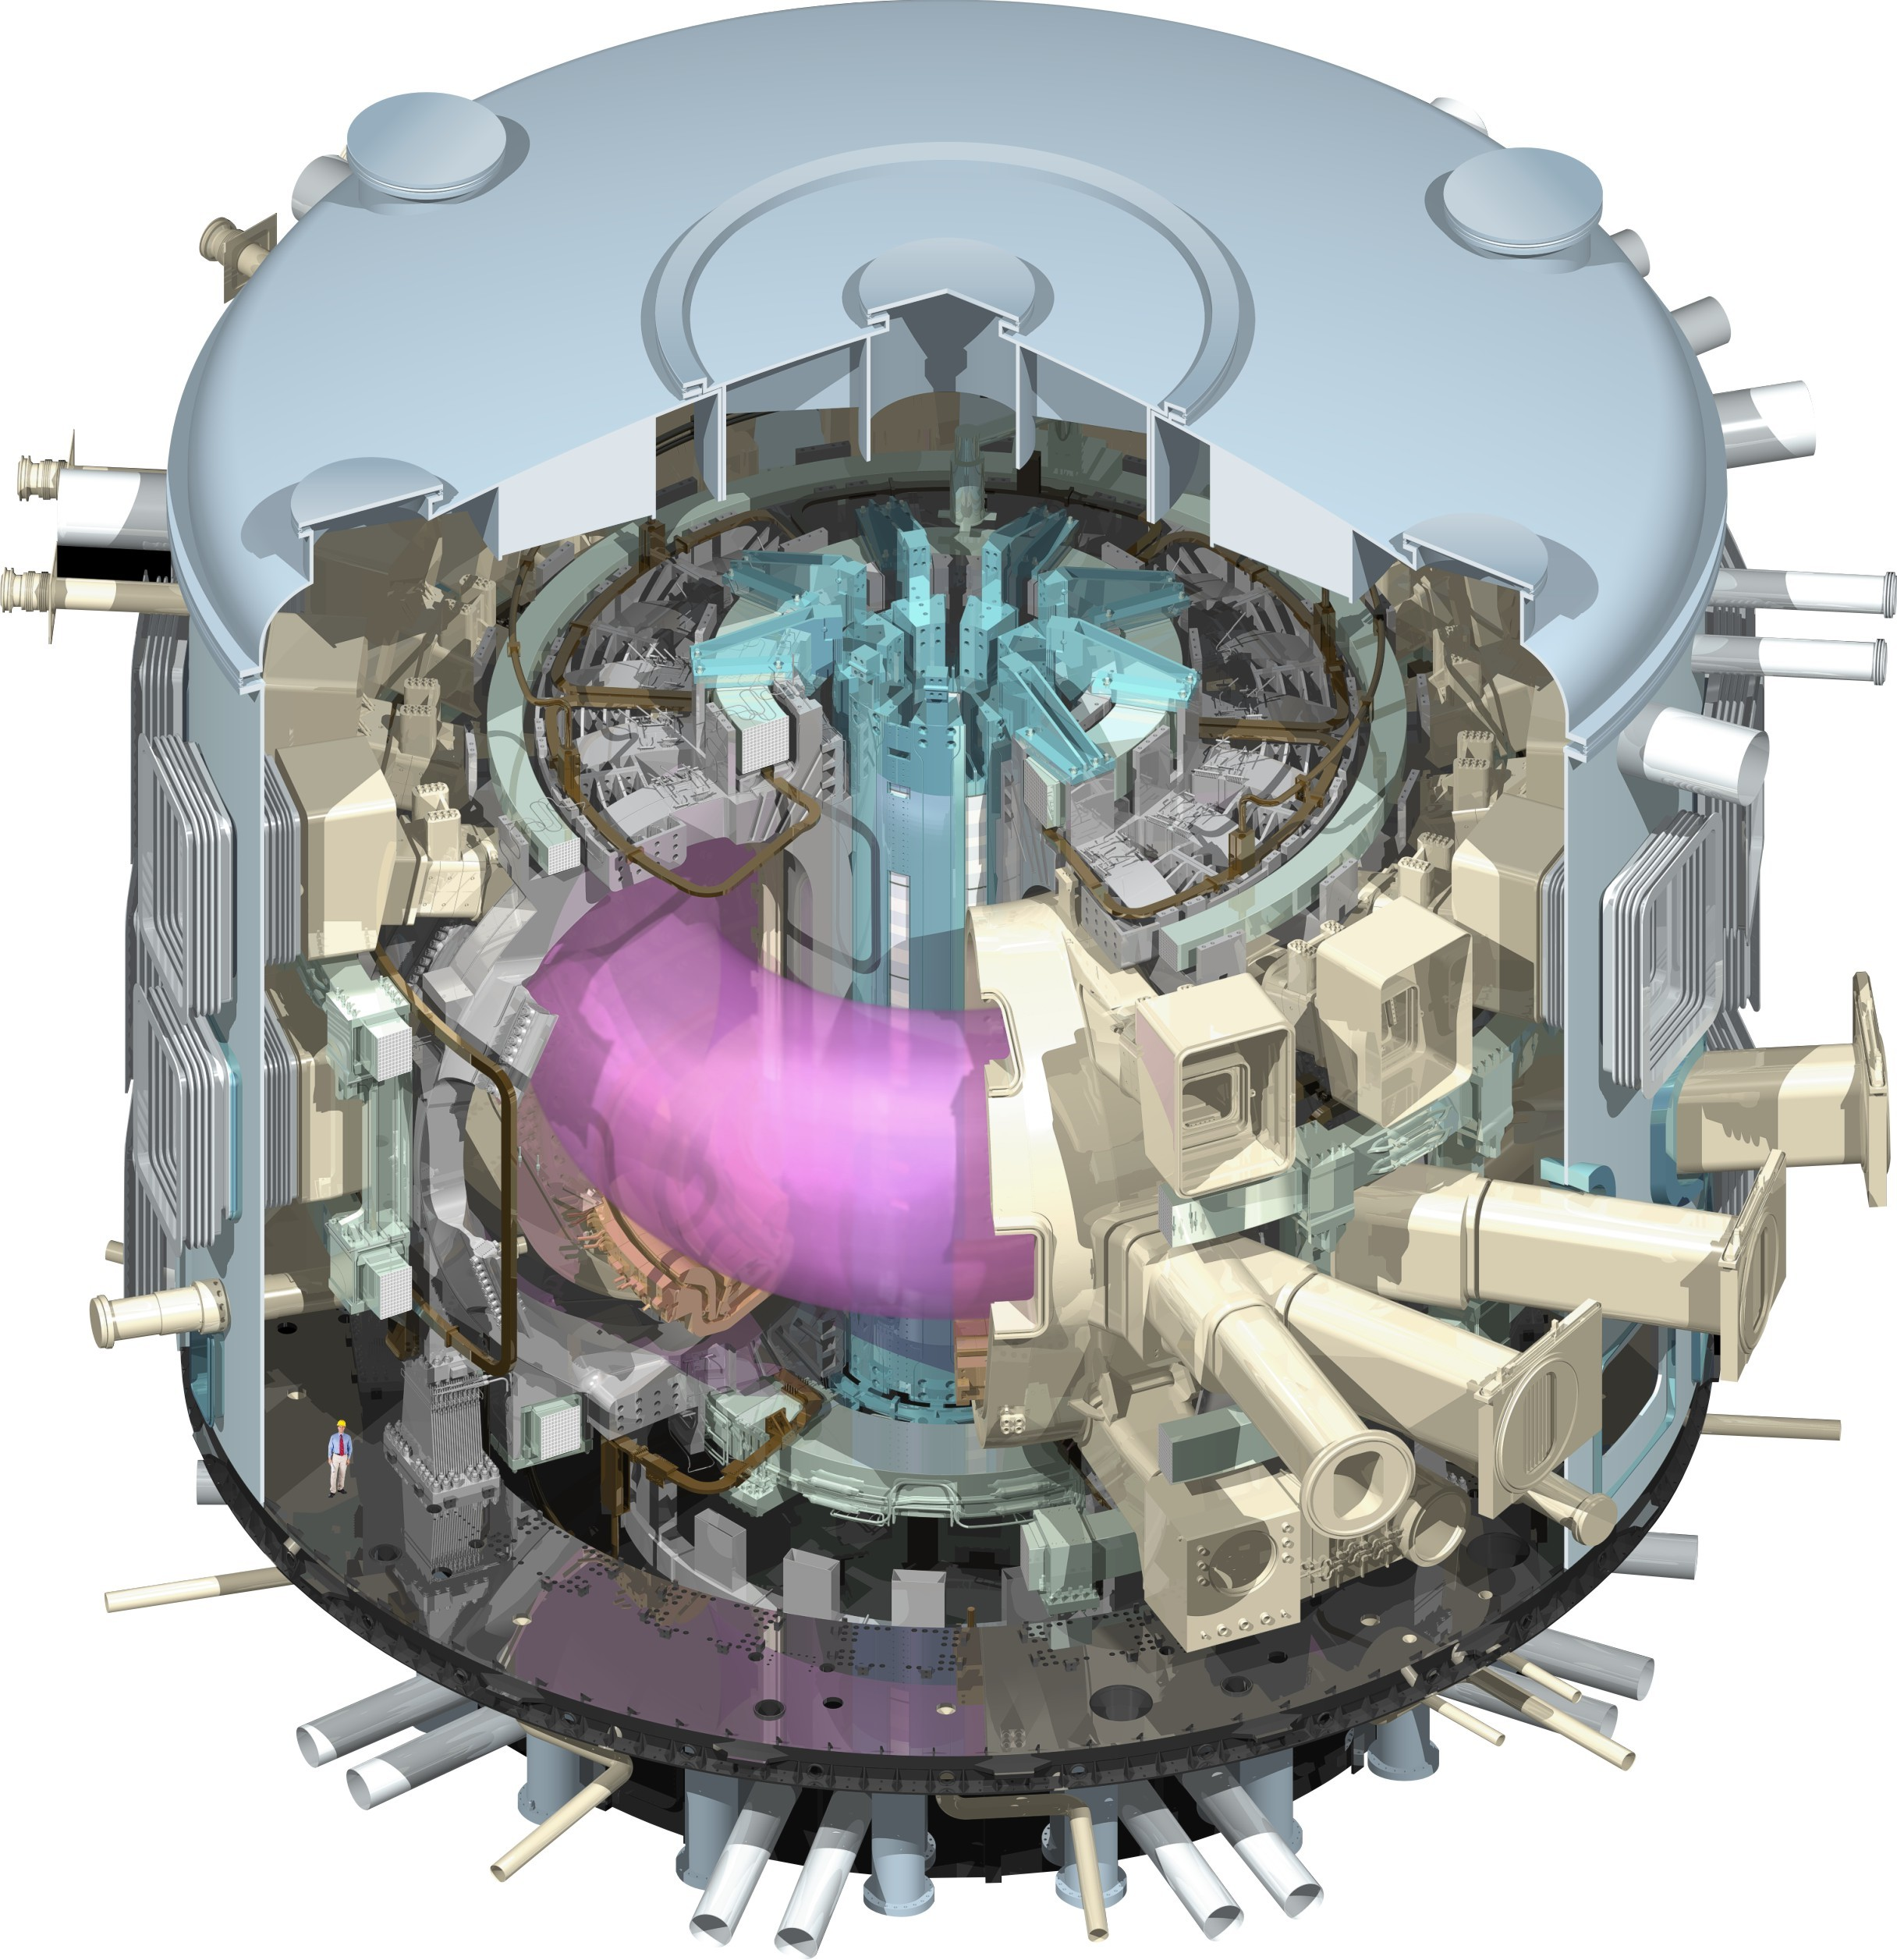
\includegraphics[width=.5\textwidth]{Figures/ITERmachine.jpg}
	\begin{description}
		\item[Abstract] Abstract
	\end{description}
\end{abstract}

\title{10401\\Fusion Energy and Plasma Physics}
\date{January \nth{24} 2019}
\author{Rasmus Kronborg Finnemann Wiuff (s163977)}
\email[E-mail at ]{s163977@student.dtu.dk}
\author{Nicklas Kihm (s143286)}
\email[E-mail at ]{spacrone@live.dk}
\affiliation{Technical University of Denmark}
\homepage[Homepage of the Technical University of Denmark ]{http://www.dtu.dk/english/}
%\homepage[\\\faGithub \ Project Code Repository: ]{https://github.com/rwiuff/Nanomechanics-for-graphene-membranes}
\maketitle

\pagenumbering{arabic}

\tableofcontents

% ToC before List-ofs fix
\makeatletter
\let\toc@pre\relax
\let\toc@post\relax
\makeatother

\thispagestyle{empty}
%\newpage
\setcounter{page}{1}

%Text
\section{Intro}
% !TEX root = ../Main.tex
In recent years a large and quickly growing collaboration between plasma physcisists and engineers have materialised into one of the most ambitious energy producing projects ever seen. The proof-of-concept plasma fusion tokamak reactor ITER\footnote{\url{https://www.iter.org/}} in Cadarache is currently taking shape in order to adress the issue of growing energy demands and climate changes.\newline The mission is simple: Prove that plasma fusion is a viable source of electricity.\newline
Whilst not being the most surmountable task, many researchers and institutions have gathered from across the world, including the Department of Physics at DTU.\newline
In this paper, three assignments are solved as part of the course ``10401 Fusion Energy and Fusion Plasma Physics''. Some key aspects of fusion plasma fueled reactors are adressed and discussed in the assignments.

\section{Part 1: A simple reactor model}
% !TEX root = ../Main.tex
\subsection{Freidberg's simple reactor model}
In the \nth{5} chapter of the textbook by Freidberg\cite{freidberg_plasma_2007}, he makes a simple model for designing a fusion reactor power plant.
The model uses simple geometric and electromagnetic assumptions with little involvement of plasma physics. The variables put into the model are shown in \cref{VFR}.
\begin{table}
	\begin{tabular}{lr}
		\toprule
		Symbol                         & Quantity                                                                                 \\
		\midrule
		\(n_\mathrm{flux \ fraction}\) & n flux in breeder end/n flux in breeder start \(\bqty{}\)                                \\
		\(C_F\)                        & Fixed cost propotionality constant \(\bqty{\$}\)                                         \\
		\(C_I\)                        & Nuclear island cost propotionality constant \(\bqty{\$\cdot\si{\watt\per\meter\cubed}}\) \\
		\(P_E\)                        & Desired output power \(\bqty{\si{\mega\watt}}\)                                          \\
		\(P_W\)                        & Maximum wall load \(\bqty{\si{\mega\watt\per\meter\squared}}\)                           \\
		\(B_{\max}\)                   & Magnetic field at the edge of the coil \(\bqty{\si{\tesla}}\)                            \\
		\(\sigma_{\max}\)              & Tensile strenght of the magnetic field coils \(\bqty{\si{\atm}}\)                        \\
		\(\eta_t\)                     & Energy conversion efficiency \(\bqty{}\)                                                 \\
		\bottomrule
	\end{tabular}
	\caption{Variables in the Freidberg's model}
	\label{VFR}
\end{table}
\cref{QFR} shows the output quantities from the model.
\begin{table}
	\begin{tabular}{llr}
		\toprule
		Symbol                    & Quantity                                                       & Obtained values                  \\
		\midrule
		\(b\)                     & Blanket-and-shield thickness                                   & \SI{1.2037}{\meter}              \\
		\(c\)                     & Magnet coil thickness                                          & \SI{0.7993}{\meter}              \\
		\(a\)                     & Minor radius                                                   & \SI{2.0098}{\meter}              \\
		\(R_0\)                   & Major radius                                                   & \SI{4.9583}{\meter}              \\
		\(A\)                     & Aspect ratio                                                   & 2.4670                           \\
		\(A_p\)                   & Plasma surface                                                 & \SI{393.4152}{\meter\squared}    \\
		\(V_p\)                   & Plasma volume                                                  & \SI{395.3509}{\meter\cubed}      \\
		\(P_\mathrm{dens}\)       & Power density                                                  & \SI{4.9685e06}{\watt\per\meter}  \\
		\(p\)                     & Plasma pressure                                                & \SI{7.3672e05}{\pascal}          \\
		\(n\)                     & Particle density                                               & \SI{1.5327e20}{\per\meter\cubed} \\
		\(B_0\)                   & Magnetic field at magnetic axis                                & \SI{4.5744}{\tesla}              \\
		\(\beta\)                 & Normalised plasma pressure                                     & 8.85\%                           \\
		\(\tau_{E_\mathrm{min}}\) & Min confinement time for \(\pqty{p\times\tau_E}_\mathrm{min}\) & \SI{1.1415}{\second}             \\
		\bottomrule
	\end{tabular}
	\caption{Output quantities in the model in Freidberg's\cite{freidberg_plasma_2007} along with the obtained values when inserting the parameters from \cref{Inputparam}}
	\label{QFR}
\end{table}
This model has been implemented in a matlab script provided for the course. The script is shown included in \cref{tokamakDTU_asign_1}.
As an example, the model is run with the following parameters:
\begin{alignat}{3}
	n_\mathrm{flux \ fraction} & = 0.01                                 & \quad P_E      & = \SI{1000}{\mega\watt} \nonumber       \\
	P_W                        & = \SI{4}{\mega\watt\per\meter\squared} & \quad B_{\max} & = \SI{13}{\tesla}    \label{Inputparam} \\
	\sigma_{\max}              & = \SI{3000}{\atm}                      & \quad \eta_t   & = 0.4 \nonumber
\end{alignat}
Note that \(C_F\) and \(C_I\) has been ommited as these serve no purpose for this assignment. It is not of interest how expensive the plant will be. Rather the geometries and physical quantities are of interest.
The results from the model is given in \cref{QFR}.
\subsection{Model sensitivity}
At this point Freidberg has provided a model that produce some reasonable results for a powerplant. It could be interesting to see how this model behaves when some vital parameters are changed. In the last section the model used the parameters shown in \cref{Inputparam}. Now the model will be iteratet over variations in the following parameters, while retaining the rest.
The variable parameters are the electric power \(P_E\), the maximum wall loading \(P_W\), the maximum magnetic field \(B_{\max}\) and the maximum stress \(\sigma_{\max}\).
\cref{IterateTokamakDTU} includes the code for iterating the matlab model over various paremeters.
\subsubsection{Change in desired power output.}
For the rise in megawatts produced (\SIrange{500}{1000}{\mega\watt}) there are a linear rise in aspect ratio, major radius, plasma surface and plasma volume. The rest of the parameters where constant except for the magnetic field strenght at the magnetic axis and the normalised plasma pressure. These are shown in \cref{PE}.

% \subsubsection{\(P_W\) \SIrange{0}{10}{\mega\watt\per\meter\squared}}
% \subsubsection{\(B_{\max}\) \SIrange{0}{20}{\tesla}}
% \subsubsection{\(\sigma_{\max}\) \SIrange{2000}{5000}{\atm}}
\subsection{Elliptic Cross section}
Freidberg's model assumes a circular cross section of the plasma. In reality this is not the case, and as of such we will now make a more realistic, yet still approximate reactor for an elliptic plasma cross section.
In describing the geometry one refers to the elongation ratio:
\begin{align}
	\kappa = \frac{a_{\max}}{a_{\min}}
\end{align}
With $a_{\max}$ the major radius and $a_{\min}$ the minor radius of the ellipse. This parameter ensures a true elliptic cross section as defined by the equation,
\begin{align}
	\frac{x^2}{a_{\max}}+\frac{y^2}{a_{\min}} = 1
\end{align}
which can be parameterised as
\begin{align}
	\mqty[x_1 \\y_1] &= \mqty[a_{\min}\cos{\phi}\\\kappa a_{\min}\sin{\phi}] \\
	\label{eq:inner_ellipse}
\end{align}
\begin{wrapfigure}[14]{r}{.4\textwidth}
	%\vspace{-5mm}
	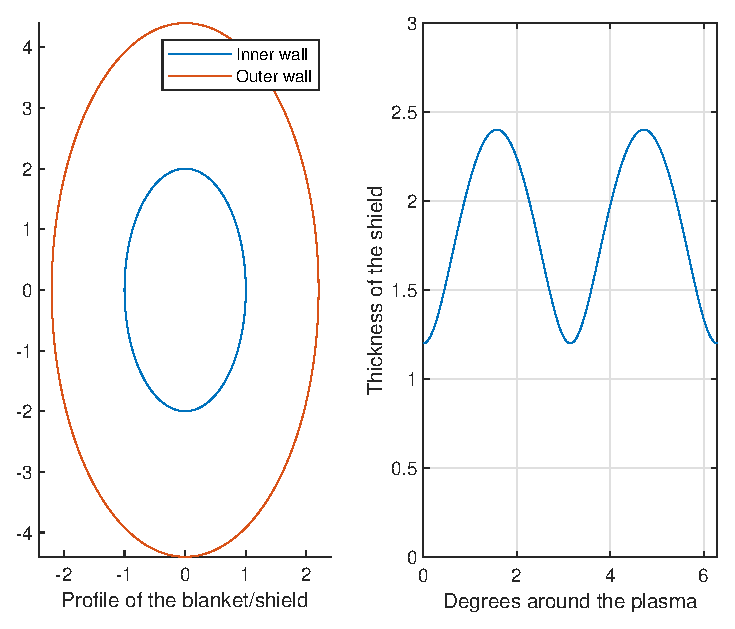
\includegraphics[width=.4\textwidth]{MatlabFigures/ShieldThickness/ShieldThickness.eps}
	\caption{The profile of the blanket-and-shield and the thickness as a function of the angle around origo, \(\phi\).}
	\label{ShTh}
\end{wrapfigure}
Meanwhile the blanket must be implemented as an ellipse or swelled ellipse. The true ellipse results in a difference of thickness in the blanket while the second results in a blanket of equal thickness throughout the structure. To this, the choice of implementing the blanket as a true ellipse has been made, since it simplifies derivations a bit. Note however, that keeping a constant thickness is the preferable option as it will reduce the engineering volume and hence the cost of the machine.\\
The outher layer is parameterised 
\begin{align}
	\mqty[x_2 \\y_2] &= \mqty[\pqty{b+a_{\min}}\cos{\phi}\\\kappa \pqty{b+a_{\min}}\sin{\phi}]
	\label{eq:outer_ellipse}
\end{align}
with $b$ the blanket thickness at the minor ellipse axis. Choosing for now, $a_{\min}=2$, $\kappa=2$ and $b=1.2$, \ref{eq:inner_ellipse} and \ref{eq:outer_ellipse} are plotted on Figure \ref{ShTh} along with the variation in thickness of the blanket. \\
Given \ref{eq:inner_ellipse} and \ref{eq:outer_ellipse}, the engineering volume can easily be derived if $c\,\cos(\phi)$ and $\kappa\, c\,\sin(\phi)$ is added to the x and y-direction in \ref{eq:outer_ellipse} respectively, where $c$ is the minimum thickness of the magnetic coils that provide the torroidal field. \\
The cross sectional area of an ellipse is $A_{\si{e}}=\pi\, a_{\min}\, a_{\max}$ so the engineered volume becomes
\begin{align}
	V_{\si{I}}=2\,\pi\, R_{0}\,(A_{\si{e,outer}}-A_{\si{e,inner}})=2\,\pi^{2}\, R_{0}\,\left(\left(a_{\min}+b+c\right)^{2}-a_{\min}^{2}\right)\,\kappa
	\label{eq:engineered_volume}
\end{align}
and the plasma volume is similarly calculated as $V_{\si{P}}=2\,\pi^2\, R_{0}\,\kappa\, a_{\min}^{2}$. The plasma surface area is a bit more tricky, but it can be approximated as
\begin{align}
	S_{\si{p}}=2\,\pi\, R_{0}\,\pi\,(3\,(a_{\min}+\kappa\, a_{\min})-\sqrt{(3\, a_{\min}+\kappa\, a_{\min})\,(a_{\min}+3\,\kappa\, a_{\min})})
\end{align}
Using the same arguments as in the book, the B-field in the centre is surprisingly unchanged when going to the elliptical model. Now c is also approximated, or rather overestimated using a slight change to eq. (5.24) in the textbook. Since the force grows with $a_{\min}$ inserting $\kappa\, a_{\min}$ instead yields an overestimation on the vertical force on the magnet. The tensile forces are the same, so the force balance leads to
\begin{align}
	c=\frac{2\,\xi}{1-\xi}(\kappa\, a+b)
\end{align}
with $\xi=B_{si{c}}^2/4\,\mu_{0}\,\sigma_{\si{max}}$. These new equations are inserted in the code. The results are displayed in \ref{tab:ellip_output}. The plasma volume and surface area is of course increased as the plasma was made higher. This of course also results in a decreased power density. Overall, parameters such as $B_{0}$, $\beta$ and $\tau_{\si{E_{\min}}}$ while changing a bit, they were not changed significantly. 

\begin{table}
	\begin{tabular}{llr}
		\toprule
		Symbol                    & Quantity                                                       & Obtained values                  \\
		\midrule
		\(b\)                     & Blanket-and-shield thickness                                   & \SI{1.2037}{\meter}              \\
		\(c\)                     & Magnet coil thickness                                          & \SI{1.2992}{\meter}              \\
		\(a\)                     & Minor radius                                                   & \SI{2.0098}{\meter}              \\
		\(R_0\)                   & Major radius                                                   & \SI{4.9583}{\meter}              \\
		\(A\)                     & Aspect ratio                                                   & 2.4670                           \\
		\(A_p\)                   & Plasma surface                                                 & \SI{608.7415}{\meter\squared}    \\
		\(V_p\)                   & Plasma volume                                                  & \SI{793.4534}{\meter\cubed}      \\
		\(P_\mathrm{dens}\)       & Power density                                                  & \SI{2.4756e06}{\watt\per\meter}  \\
		\(p\)                     & Plasma pressure                                                & \SI{5.2003e05}{\pascal}          \\
		\(n\)                     & Particle density                                               & \SI{1.0819e20}{\per\meter\cubed} \\
		\(B_0\)                   & Magnetic field at magnetic axis                                & \SI{4.6037}{\tesla}              \\
		\(\beta\)                 & Normalised plasma pressure                                     & 6.17\%                           \\
		\(\tau_{E_\mathrm{min}}\) & Min confinement time for \(\pqty{p\times\tau_E}_\mathrm{min}\) & \SI{1.6172}{\second}             \\
		\bottomrule
	\end{tabular}
		\caption{Output quantities from the elliptical model}
	\label{tab:ellip_output}
\end{table}




\subsection{Main parameters for DEMO}

Setting $P_{\si{E}}=2000$ in the elliptical model yields the output parameters seen in table \ref{tab:DEMO}. Since $R_{0}$ is directly proportional to the electric power this of course increases linearly. The other geometric output parameters regarding areas and volumes also increase as a result. $\beta$ has decreased a lot, so the plasma is not confined effectively in DEMO.

\begin{table}
	\begin{tabular}{llr}
		\toprule
		Symbol                    & Quantity                                                       & Obtained values                \\
		\midrule
		\(b\)                     & Blanket-and-shield thickness                                   & \SI{1.2037}{\meter}              \\
		\(c\)                     & Magnet coil thickness                                          & \SI{1.2992}{\meter}              \\
		\(a\)                     & Minor radius                                                   & \SI{2.0098}{\meter}              \\
		\(R_0\)                   & Major radius                                                   & \SI{9.9510}{\meter}              \\
		\(A\)                     & Aspect ratio                                                   & 4.9512                           \\
		\(A_p\)                   & Plasma surface                                                 & \SI{1.21175e03}{\meter\squared}   \\
		\(V_p\)                   & Plasma volume                                                  & \SI{1.5869e03}{\meter\cubed}     \\
		\(P_\mathrm{dens}\)       & Power density                                                  & \SI{2.4756e06}{\watt\per\meter}  \\
		\(p\)                     & Plasma pressure                                                & \SI{5.2003e05}{\pascal}          \\
		\(n\)                     & Particle density                                               & \SI{1.0819e20}{\per\meter\cubed} \\
		\(B_0\)                   & Magnetic field at magnetic axis                                & \SI{8.8018}{\tesla}              \\
		\(\beta\)                 & Normalised plasma pressure                                     & 1.69\%                         \\
		\(\tau_{E_\mathrm{min}}\) & Min confinement time for \(\pqty{p\times\tau_E}_\mathrm{min}\) & \SI{1.6172}{\second}             \\
		\bottomrule
	\end{tabular}
	\caption{Output quantities for DEMO using the elliptical model with $P_{\si{E}}=2\si{GW}$}
	\label{tab:DEMO}
\end{table}

\subsection{Designs for DEMO}

With $P_{\si{E}}$, $\kappa=2$ and $A=R_{0}/a_{\min}=3\Leftrightarrow R_{0}=3\, a_{\min}$. This is implemented in the code and the results are displayed in \ref{tab:DEMO2}. $\beta$ has increased a bit but only to $4.55\%$. $R_{0}$ has been forced down, so the plasma volume etc. has decreased as well. Overall it seems like a smaller $R_{0}$ while keeping $a_{min}$ fixed is an improvement. Or in other words, $A=3$ is more desirable than $A\approx 5$. 

\begin{table}
	\begin{tabular}{llr}
		\toprule
		Symbol                    & Quantity                                                       & Obtained values                \\
		\midrule
		\(b\)                     & Blanket-and-shield thickness                                   & \SI{1.2037}{\meter}              \\
		\(c\)                     & Magnet coil thickness                                          & \SI{1.2992}{\meter}              \\
		\(a\)                     & Minor radius                                                   & \SI{2.0098}{\meter}              \\
		\(R_0\)                   & Major radius                                                   & \SI{6.0295}{\meter}              \\
		\(A\)                     & Aspect ratio                                                   & 3                              \\
		\(A_p\)                   & Plasma surface                                                 & \SI{737.6961}{\meter\squared}   \\
		\(V_p\)                   & Plasma volume                                                  & \SI{961.5370}{\meter\cubed}         \\
		\(P_\mathrm{dens}\)       & Power density                                                  & \SI{4.0857e06}{\watt\per\meter}  \\
		\(p\)                     & Plasma pressure                                                & \SI{6.6807e05}{\pascal}          \\
		\(n\)                     & Particle density                                               & \SI{1.3899e20}{\per\meter\cubed} \\
		\(B_0\)                   & Magnetic field at magnetic axis                                & \SI{6.0714}{\tesla}              \\
		\(\beta\)                 & Normalised plasma pressure                                     & 4.55\%                         \\
		\(\tau_{E_\mathrm{min}}\) & Min confinement time for \(\pqty{p\times\tau_E}_\mathrm{min}\) & \SI{1.2588}{\second}             \\
		\bottomrule
	\end{tabular}
	\caption{Output quantities for DEMO using the elliptical model with $P_{si{E}}=2$, $\kappa=2$ and setting $A=3$}
	\label{tab:DEMO2}
\end{table}

\subsection{\textit{A} and \mathinhead{\kappa}{\kappa} as free parameters}

Designing the tokamak with $\kappa$ and $A$ as free parameters has led us to try and maximise profitability from $V_{P}/A_{P}$ and $\beta$. Profitability in this context means that increasing the size of the tokamak leads to an increase in these parameters. However, there is a point when the change vs increase in size becomes constant. This means that we do not profit from increasing the size any longer. \\
$V_{\si{P}}$ and $A_{\si{P}}$ were calculated earlier so
\begin{align}
    \frac{V_{\si{P}}}{A_{\si{P}}}=\frac{2\,\pi\, R_{0}\,\kappa\, a_{\min}^{2}}{2\,\pi\, R_{0}\,\pi\, (3\,(a+\kappa\, a_{min})-\sqrt{(3\, a_{\min}+\kappa\, a_{\min})\,(a+3\,\kappa\, a_{\min})})}=\frac{\kappa\, a_{\min}}{\pi\,(3+3\,\kappa-\sqrt{3+\kappa}\,\sqrt{1+3\,\kappa})}
\end{align}
The expression scales linearly with $a_{min}$ so we set it equal to $1\si{m}$ since it has no effect on the choice of $\kappa$. Differentiating with respect to $\kappa$ and plotting is done, with the results shown in Figure \ref{kappa_change}. Considering the figure, $\kappa=2.5$ is chosen as the change is close enough to zero given this value.\\
Now work will be done towards choosing a value for $A$. First for geometric reasons a minimum $R_{0}$ is calculated. It is simply $R_{0}=a_{\min}+b+c$ where $a_{min}$ is to be determined, $b=1.2\si{m}$ and $c=\frac{2\,\xi}{1-\xi}(\kappa\, a_{\min}+b)$. Meanwhile $A$ is chosen to optimize $\beta$. Inserting $R_{0}$ into $B_{0}$ in the textbook yields
\begin{align}
    B_{0}=\frac{2\,\xi\,(\kappa\, a_{\min}+b)\, B_{max}}{((2\,\kappa-1)\, a_{\min}+a+b)}=\frac{178.75\, a_{\min}+85.8}{55.5+36\, a_{\min}}
\end{align}
Where units has been disregarded and $\xi=0.11$, $b=1.2$, $\kappa=2.5$ and $B_{\si{max}}=13$ has been inserted. Meanwhile, inserting the textbook's expression for $P_{\si{dens}}$ into the expression for $p$ and inserting the input parameters yields
\begin{align}
    p=1.042\si{E}6\,\sqrt{\frac{1}{\kappa\, a_{\min}}}
\end{align}
Thus $\beta$ becomes
\begin{align}
    \beta=\frac{2148\,(a_{\min}+1.542)^{2}}{\sqrt{a_{\min}}\,(178.8\, a_{\min}+85.8)^{2}}
\end{align}
This function is plotted in Figure \ref{beta_vs_a} and for $\beta=10\‰$ $a=1.938\si{m}$ is achieved. Therefore $R_{0}=1.9378\si{m}+1.2\si{m}+2\cdot 0.11/(1-0.11)\cdot 2.5\cdot 1.938\si{m}+1.2\si{m}=4.632\si{m}$ which means $A=4.632\si{m}/1.938\si{m}=2.390$





\begin{figure}
	\centering
	\begin{subfigure}[h!]{.40\textwidth}
		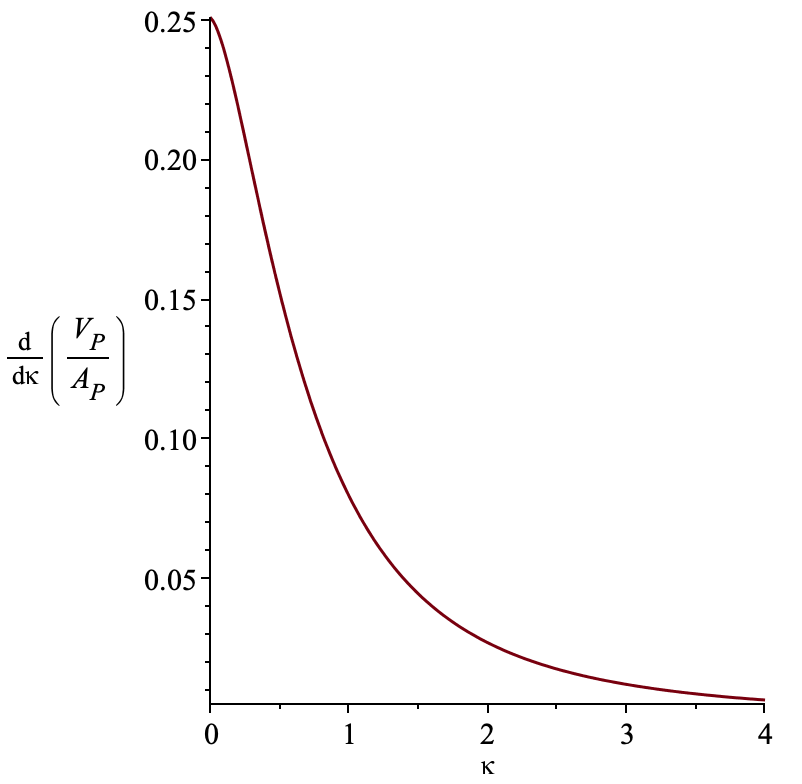
\includegraphics[width=\textwidth]{Figures/kappa_change.png}
		\caption{}
		\label{kappa_change}
	\end{subfigure}
	~
	\begin{subfigure}[h!]{.40\textwidth}
		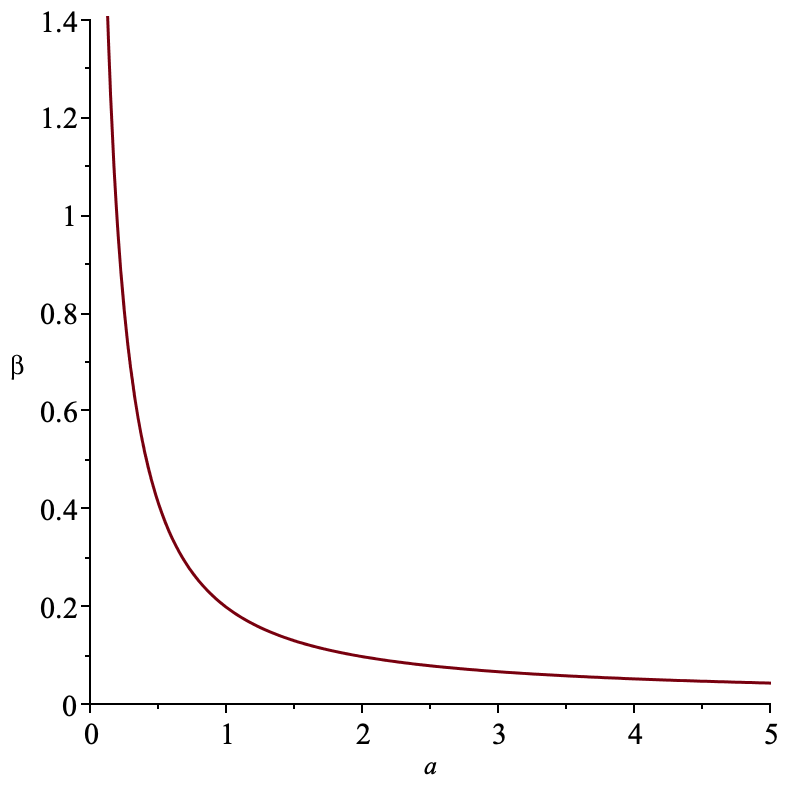
\includegraphics[width=\textwidth]{Figures/beta_vs_a.png}
		\caption{}
		\label{beta_vs_a}
	\end{subfigure}
	\caption{}
	\label{A_kappa}
\end{figure}

\begin{table}
	\begin{tabular}{llr}
		\toprule
		Symbol                    & Quantity                                                       & Obtained values                \\
		\midrule
		\(b\)                     & Blanket-and-shield thickness                                   & \SI{1.20}{\meter}              \\
		\(c\)                     & Magnet coil thickness                                          & \SI{1.30}{\meter}              \\
		\(a\)                     & Minor radius                                                   & \SI{2.01}{\meter}              \\
		\(R_0\)                   & Major radius                                                   & \SI{2.60}{\meter}              \\
		\(A\)                     & Aspect ratio                                                   & 1.29                           \\
		\(A_p\)                   & Plasma surface                                                 & \SI{630}{\meter\squared}       \\
		\(V_p\)                   & Plasma volume                                                  & \SI{414}{\meter\cubed}         \\
		\(P_\mathrm{dens}\)       & Power density                                                  & \SI{9.49e06}{\watt\per\meter}  \\
		\(p\)                     & Plasma pressure                                                & \SI{1.02e05}{\pascal}          \\
		\(n\)                     & Particle density                                               & \SI{2.12e20}{\per\meter\cubed} \\
		\(B_0\)                   & Magnetic field at magnetic axis                                & \SI{-3.09}{\tesla}             \\
		\(\beta\)                 & Normalised plasma pressure                                     & 26.9\%                         \\
		\(\tau_{E_\mathrm{min}}\) & Min confinement time for \(\pqty{p\times\tau_E}_\mathrm{min}\) & \SI{1.26}{\second}             \\
		\bottomrule
	\end{tabular}
	\caption{Output quantities for the elliptical model after $\beta$ and $A$ has been optimised}
	\label{tab:DEMO3}
\end{table}







%, even after increasing the radii to accomodate the larger ellipses describing the blanket-and-shield. This does however mean that the fixed thickness, \(b\) from Freidberg's model is variable. To find this variation the parametric ellipses defining the blanket-and-shield are defined with \(b\) being the length difference between the larger radii and the length difference between the smaller radii.
%\begin{wrapfigure}[14]{r}{.4\textwidth}
%\vspace{-5mm}
%	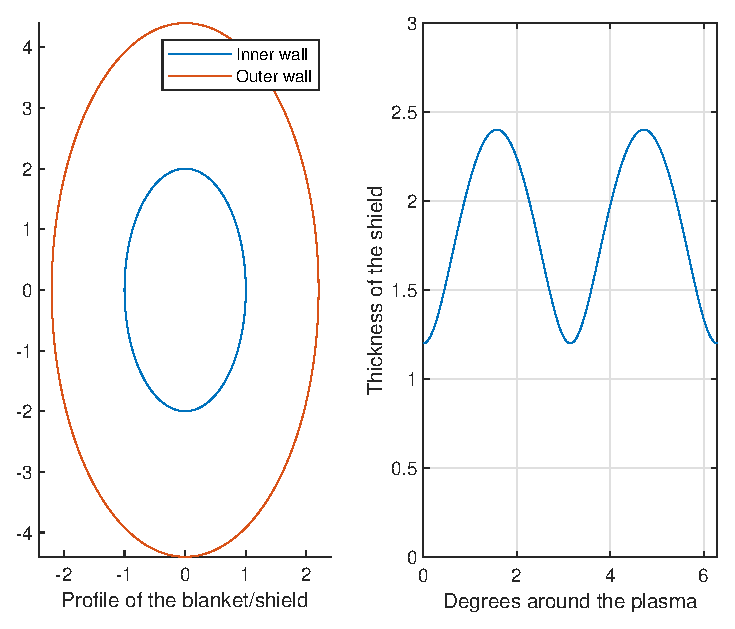
\includegraphics[width=.4\textwidth]{MatlabFigures/ShieldThickness/ShieldThickness.eps}
%	\caption{The profile of the blanket-and-shield and the thickness as a function of the angle around origo, \(\phi\). The parameters here are given in \cref{ellparam}}
%	\label{ShTh}
%\end{wrapfigure}
%\begin{align}
%	\mqty[x_1 \\y_1] &= \mqty[a_{\min}\cos{\phi}\\\kappa a_{\min}\sin{\phi}] \\
%	\mqty[x_2 \\y_2] &= \mqty[\pqty{b+a_{\min}}\cos{\phi}\\\kappa \pqty{b+a_{\min}}\sin{\phi}]
%\end{align}
%At a given angle, \(\phi\), the distance must be:
%\begin{align}
%	\vb{u}-\vb{v}       & = \mqty[\cos{\phi}b                                  \\\kappa\sin{\phi}b] \\
%	\abs{\vb{u}-\vb{v}} & = \sqrt{\cos^2{\phi}\ b^2+\kappa^2\sin^2{\phi}\ b^2}
%\end{align}
%An example is given in \cref{ShTh}. Here the parameters are:
%\begin{alignat}{3}\label{ellparam}
%	\mqty{a_{\min} \\\kappa\\b}&\ \mqty{=\\=\\=}\ &\mqty{2\\2\\1.2}
%\end{alignat}

\section{Part 2: Diagnostics via interferometry}
% !TEX root = ../Main.tex
When operating a fusion reactor a continuous process of diagnostics is necessary in order to optimise the plasma for the fusion process. One of the active diagnostic methods are interferometry.
The goal here for this part of the paper is to measure the plasma electron density in the Danish Tokamak Undertaking reactor.
\subsection{Cut-off and Source frequency}
Using a interferometer one can measure the electron density \(n_e\) of the plasma. The refractive index of electromagnetic waves depend on the electron density and plasma frequency \(\omega_p\) proportionally:
\begin{align}
	\omega_p^2 \propto n_e
\end{align}
For O-mode plasma waves, the refractive index is:
\begin{align}
	N_{\mathrm{O}} = \sqrt{1-\frac{\omega_p^2}{\omega^2}}
\end{align}
with \(\omega\) being the probing wave frequency.
The plasma will reflect the beam if the plasma frequency is larger than the beam frequency so
\begin{align}
	\omega > \omega_p = \sqrt{n_e\frac{e^2}{\epsilon_0 m_{e0}}}
\end{align}
So for a given frequency, the plasma must not exceed a critical cut off electron density:
\begin{align}
	n_e < n_c      & = \omega^2\frac{\epsilon_0\cdot m_{e0}}{e^2} \label{nenc} \\
	               & \qq*{which gives} \nonumber                               \\
	N_{\mathrm{O}} & = \sqrt{1-\frac{n_e}{n_c}}\label{NO}
\end{align}
With a probing frequency much higher than the plasma frequency and the critical density much higher than the electron density \cref{NO} can be approximated by:
\begin{align}
	N_{\mathrm{O}} & = \sqrt{1-\frac{n_e}{n_c}} \approx 1-\frac{1}{2}\frac{n_e}{n_c} -\frac{\omega_p^2}{2\omega^2}
\end{align}

With sufficient accuracy, the linear dependence of the O-mode refractive index on the electron density is obtained if the normalised quantities obey:
\begin{align}
	\frac{n_e}{n_c} \leq 0.4 \quad \frac{\omega_p}{\omega} \leq 0.6
\end{align}
We must calculate the phase shift as one beam travels in vacuum by the length \(L_V\) and one wave travels in the plasma by the length \(L_P\). The phase shift in terms of \(2 \pi\) is equal to the optical difference divided by the wavelength. With the refractive index in vacuum, \(N_V=1\), this yields:
\begin{align}
	\frac{\Phi}{2\pi} & = \frac{\Delta L_{opt}}{\lambda} = \frac{\int_{x_1}^{x_2}\pqty{N_V-N_{\mathrm{O}}(x')}\dd{x'}}{\lambda} \approx \frac{1}{2\lambda n_c}\int_{0}^{x}n_e(x')\dd{x'} \nonumber \\
	                  & = 4.48\times 10^{-16} \pqty{\frac{\lambda}{\si{\meter}}}\int_{0}^{x}\pqty{\frac{n_e(x')}{\si{\per\meter\cubed}}}\pqty{\frac{\dd{x'}}{\si{\meter}}} \label{Phipi}
\end{align}
Assuming a Gaussian distribution, the electron density at \(\pm\infty\) is approximately equal to the densities just inside the reactor walls. Therefore
\begin{align}
	\int_{-\infty}^{\infty}n_e \exp\pqty{-\frac{(y-b)^2}{2c^2}}\dd{y} \approx n_e\ c\ \sqrt{2\pi}\label{c}
\end{align}
With the density at the centre given as:
\begin{align}
	\SI{e16}{\per\meter\cubed} \leq n_e \leq \SI{e18}{\per\meter\cubed},
\end{align}
The \(c\) in \cref{c} is the width of the Gaussian distribution and must fit inside the reactor. The DTU tokamak has a minor diameter of \SI{0.25}{\meter}. Thus
\begin{align}
	\frac{\Phi}{2\pi} \approx 4.48\times 10^{-16}\pqty{\frac{\lambda}{\si{\meter}}}n_e\SI{0.25}{\meter}\sqrt{2\pi} & = 1.12\times 10^{-16}\ n_e  \pqty{\frac{\sqrt{2\pi} c}{\omega\si{\meter}}} \nonumber \\
	                                                                                                               & = 8.416\times 10^{-8}\pqty{\frac{n_e}{\omega\si{\second}}}\label{Phipi2}
\end{align}
Remembering \cref{nenc}
\begin{align}
	\omega^2\frac{\epsilon_0\ m_{e0}}{e^2} & = \omega^2\frac{\SI{8.854e-12}{\farad\per\meter}\ \SI{9.109e-31}{\kilo\gram}}{\SI{1.602e-19}{\coulomb}} \\
	                                       & \Downarrow\nonumber                                                                                     \\
	n_e                                    & < 0.000314\omega^2 \label{co}
\end{align}
Where any units has been disregarded. We want the largest possible phase shift which means that the lower the frequency the better. However cutoff must first be taken into account.
Since the cutoff is given by \cref{co} and since we want to measure densities up to \SI{e18}{\per\meter\cubed} the minimum frequency of the wave is
\begin{align}
	\frac{\omega}{2\pi} & > \frac{\sqrt{\frac{\SI{e18}{\per\meter\cubed}}{0.000314}}}{2\pi} \\
	                    & \Downarrow\nonumber                                               \\
	f                   & \approx \SI{9}{\giga\hertz}
\end{align}
Given the available emitters, the best emitter is therefore the one with \(f=60\si{GHz}\).
\subsection{Beam Phase shifts}
\begin{wrapfigure}[12]{r}{.5\textwidth}
	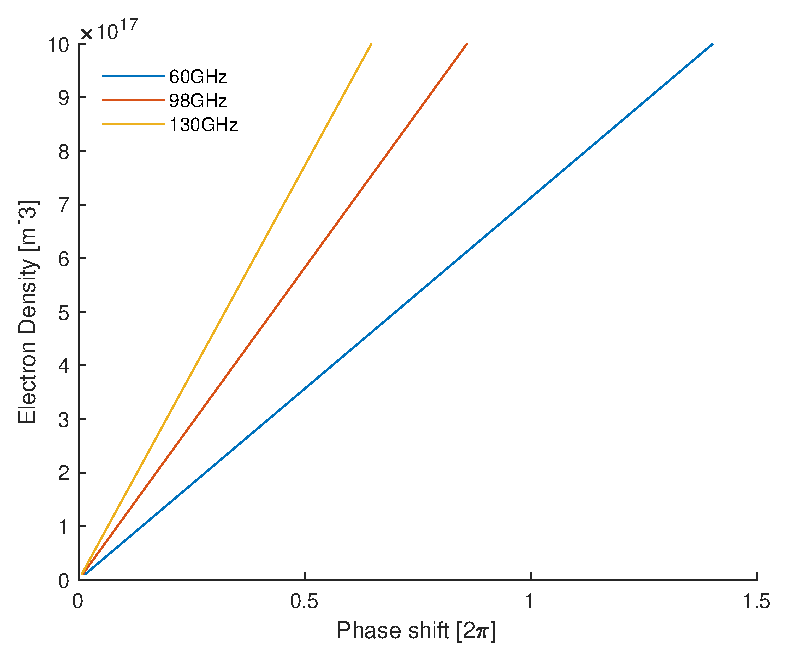
\includegraphics[width=.5\textwidth]{MatlabFigures/PhaseShift/PhaseShift.eps}
	\caption{Electron densities for different wavelengths and phase shifts}
	\label{PhPlot}
\end{wrapfigure}
The goal of the interferometer is to find the phase shift between the microwave beam in vacuum and in plasma. Our suggestion is a setup involving a interferometer emitting a beam through the centre of the reactor. The first measurement would be through vacuum to find the source phase. Afterwards phase measurements can be conducted with an active plasma in the reactor.
So by first measuring the phase of the probing beam in vacuum, one can simply measure the phase shift.\\
We know from \cref{Phipi,c,,Phipi2} that:
\begin{align}
	\frac{\Phi}{2\pi} = 8.416\times 10^{-8}\pqty{\frac{n_e}{\omega\si{\second}}}
\end{align}
So for different average electron densities through the plasma, one can plot the resulting phase shifts.
Using the code in \cref{PSD} the plot in \cref{PhPlot} is generated. The measured phase shift is then correlated to an electron density using \cref{PhPlot}.
\subsection{Evolving beam width}
\begin{wrapfigure}[14]{r}{.4\textwidth}
	\vspace{-5mm}
	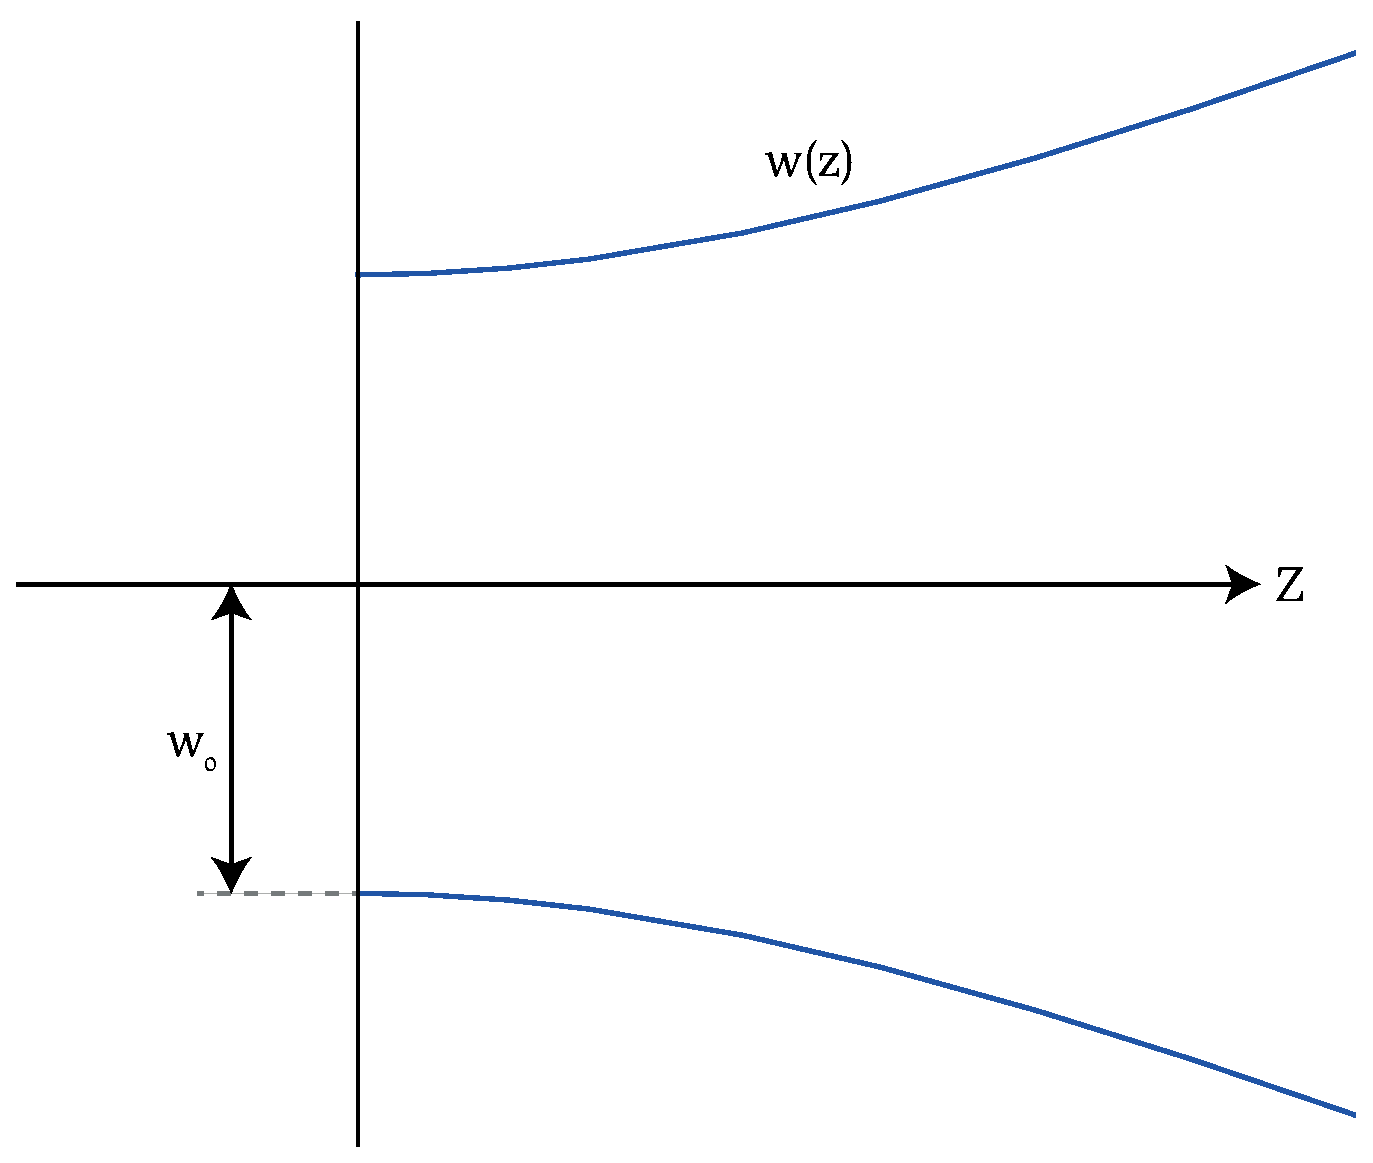
\includegraphics[width=.4\textwidth]{Figures/PropEx.eps}
	\caption{Sketch of Gaussian beam propagation with indication of \(w_0\) and \(w(z)\).}
	\label{PropEx}
\end{wrapfigure}
In our case we want to use a Gaussian microwave. Such beam propagates spatially as shown in \cref{PropEx}.
\(w_0\) is the initial beam waist determined by the source, and \(w(z)\) is the function describing the waist. This equation is:
\begin{align}
	w(z) = w_0(z)\sqrt{1+\pqty{\frac{\lambda z}{\pi w_0^2}}^2}\label{wz}
\end{align}
From this equation one can track the spatial propagation of the wave. In this project three sources are given. The initial beam waist is set to \(w_0=\SI{0.0275}{\meter}\) corresponding to half a reactor port. With
\begin{align}
	\frac{\lambda z}{\pi w_0^2} = \frac{9.543\times10^7 z}{w_0^2 f}
\end{align}
, and \(f\) the frequency of the emitter, the sources' beam waists are given as such:
\begin{align}
	\SI{60}{\giga\hertz}  & : \quad w(z)=0.0275\sqrt{\pqty{1+\frac{9.543\times10^7 z}{0.0275^2 \ 60\times10^9}}^2}\label{60}   \\
	\SI{98}{\giga\hertz}  & : \quad w(z)=0.0275\sqrt{\pqty{1+\frac{9.543\times10^7 z}{0.0275^2 \ 98\times10^9}}^2}\label{98}   \\
	\SI{130}{\giga\hertz} & : \quad w(z)=0.0275\sqrt{\pqty{1+\frac{9.543\times10^7 z}{0.0275^2 \ 130\times10^9}}^2}\label{130}
\end{align}
For the three given sources in this project, the beam waist has been plotted on \cref{BeamProp}
\newline

\begin{figure}[H]
	\centering
	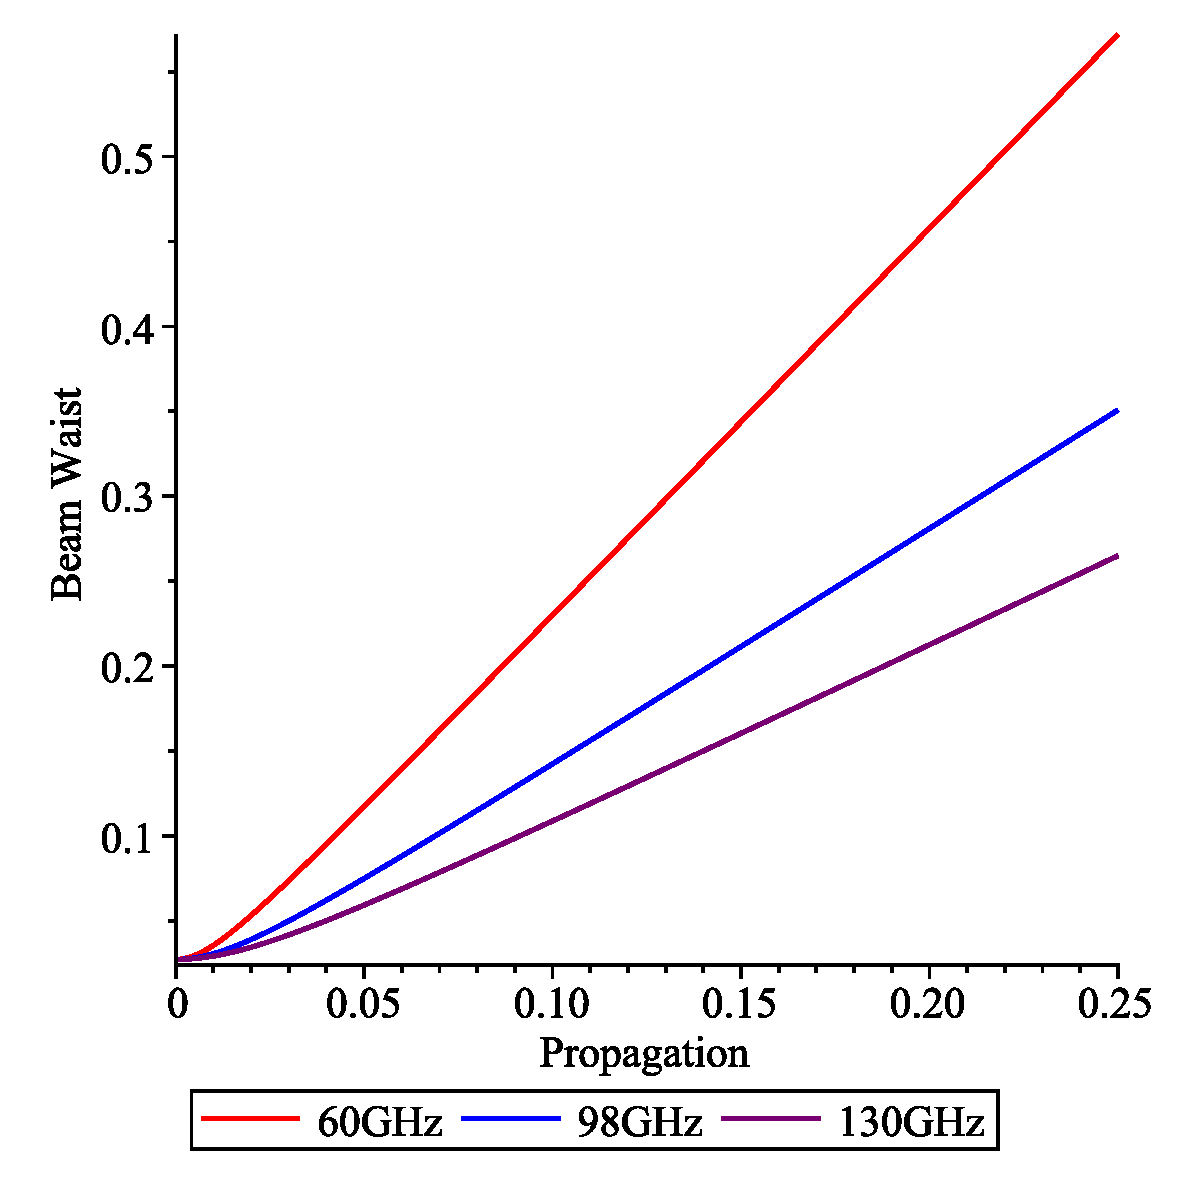
\includegraphics[width=.5\textwidth]{Figures/BeamProp.eps}
	\caption{Beam Waist for the three microwave sources. The functions are \cref{60,98,,130}.}
	\label{BeamProp}
\end{figure}
It is undesirable for some of the beam to not reach the output port and instead propagate into the reactor wall, as this will result in a lesser signal strength. Therefore it can be necessary to deploy a Gaussian telescope.
\subsection{Gaussian beam telescope interferometer}
In order to control the beam waist, one can use a Gaussian beam telescope arrangement around the reactor. A lens is placed between the source and the reactor input port and again between the output port and the receiver. From chapter 5 in ``Fusion Plasma Diagnostics with mm-Waves''\cite{PlasmaDiagnosis} the authors explains how such an arrangement can be obtained. Starting with the focal lengths of the lenses,
\begin{align}
	d = f_0 + f_1
\end{align}
, where \(f_0\) and \(f_1\) are focal lengths, and \(d\) are the distance between the lenses.
The resulting narrowest beam waist after the second lens are given as:
\begin{align}
	w_2 = \frac{f_1}{f_0}w_0
\end{align}
The use of two lenses make the transformation wavelength independent (Eq 5.118)\cite{PlasmaDiagnosis}, thus the only interaction with the wavelength of the probing beam will be that of the plasma itself.
The distance to the minimum waist after the second lens is given as:
\begin{align}
	d_3 = \frac{f_1}{f_0}\pqty{f_0+f_1-\frac{f_1}{f_0}d_0}
\end{align}
The waist in between the lenses is given as:
\begin{align}
	w_1 = \frac{\lambda f_0}{\pi w_0}
\end{align}
And the distance from the first lens to this waist is:
\begin{align}
	d_1 = \pqty{\frac{\frac{d_0}{f_0}-1}{\frac{w_0^2\pi}{f_0\lambda}+\pqty{\frac{d_0}{f_0}-1}^2}+1}f_0
\end{align}
Thus the distance from \(w_1\) to the second lens is:
\begin{align}
	d_2 = d-d_1
\end{align}
Knowing these variables and utilising \cref{wz} we can model a complete setup. Using the Matlab code in \cref{inter}, the following parameters are used:
\begin{align}
	\mqty{r_p = \SI{0.055}{\meter} & r = \SI{0.125}{\meter}  & w_0 = \SI{0.0275}{\meter} & freq = \SI{60}{\giga\hertz}        \\
	d_0 = \SI{0.20}{\meter}        & d_r = \SI{0.10}{\meter} & f_0 = \SI{0.25}{\meter}   & \SI{0.20}{\meter}} \label{interin}
\end{align}
With \(r_p\) being the tokamak port radius, \(r\) the tokamak minor radius and \(d_r\) the distance between the first lens and the reactor wall.
In the case of the Danish Tokamak Undertaking, two ports opposing each other is ideal for use with interferometry. In this example, the port radius, \(r_p\), and the minor radius \(r\) are based on the ST-25 in the basement of building 309 at DTU.
The script gave the results:
\begin{align}
	\mqty{w_1 = \SI{0.0145}{\meter} & w_2 = \SI{0.0220}{\meter}                                            \\
	d_1 = \SI{0.2243}{\meter}       & d_2 = \SI{0.2257}{\meter} & d_3 = \SI{0.232}{\meter}}\label{interou}
\end{align}
Furthermore the code plots a sketch of the desired interferometer setup. The sketch can be seen in \cref{AWESOME}.\newline
\begin{figure}
	\centering
	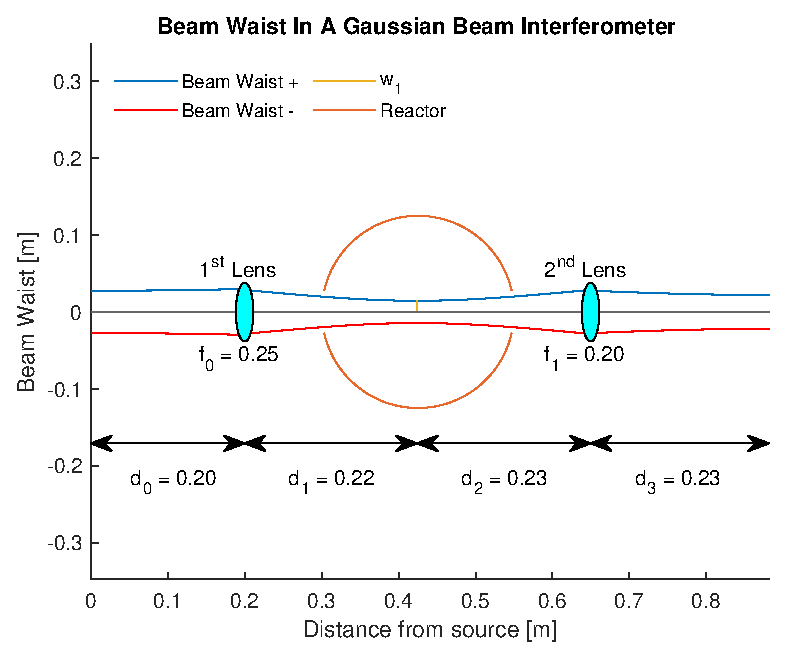
\includegraphics[width=.7\textwidth]{MatlabFigures/Interferometer/Interferometer.eps}
	\caption{Gaussian beam telescope interferometer setup with input parameters shown in \cref{interin} and output parameters shown in \cref{interou}}
	\label{AWESOME}
\end{figure}
\begin{wrapfigure}[14]{r}{.3\textwidth}
	\centering
	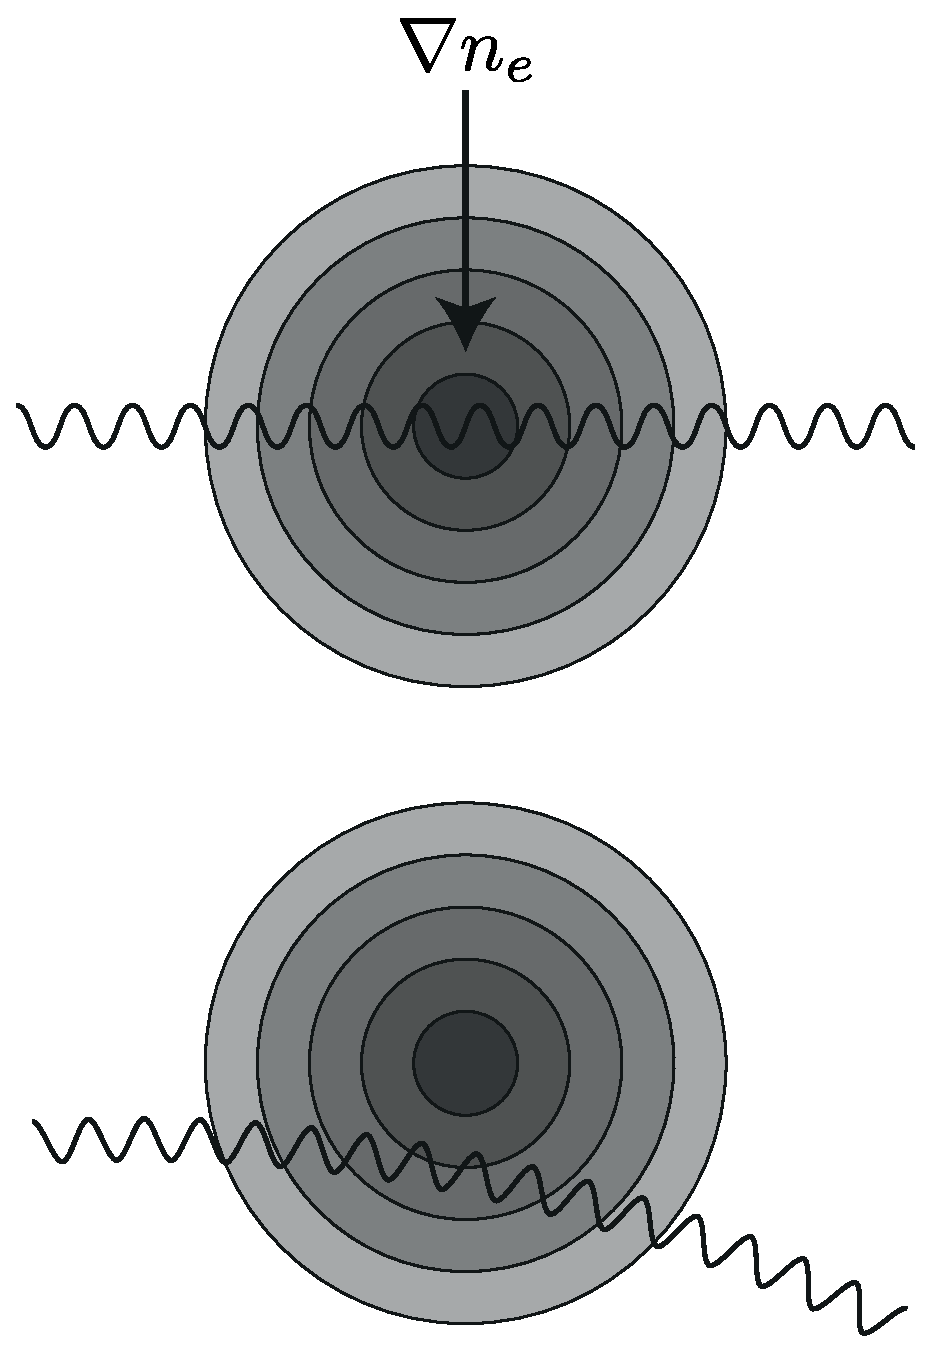
\includegraphics[width=.3\textwidth]{Figures/Refraction.eps}
	\caption{Refraction of the probing beam at centre  (top) and off centre (bottom).}
	\label{Refrac}
\end{wrapfigure}
Lastly it should be mentioned that the beam waist confinement does not matter if the wave is refracted into the side of the reactor. As the plasma density varies from the centre and out, the plasma itself act as a variable lens with variable refractive indices. If the beam is emitted straight through the centre, the refractive indices will only shorten and lengthen the wavelength back to normal, however if the beam is emitted off centre, it will be refracted away from the centre. In such a setup, further calculations need to be conducted to determine variation in signal strength, phase and wavelength. The two described setups are depicted on \cref{Refrac}.

\begin{acknowledgments}
	The authors would like to thank...
\end{acknowledgments}
%End of text

%Bibliography herunder:
\newpage
\onecolumngrid
\bibliography{Bibliography}

\newpage
\listoffigures
\listoftables
\listoflistings
%\listoftodos
\newpage
%Appendicer herunder:
% !TEX root = Main.tex
\appendix
\appendixpage
\addappheadtotoc
\section{tokamakDTU\textunderscore asign\textunderscore 1}\label{tokamakDTU_asign_1}
\inputminted[bgcolor=Black,linenos=true]{matlab}{Listings/tokamakDTU_asign_1.m}\newpage
\section{IterateTokamakDTU}\label{IterateTokamakDTU}
\inputminted[bgcolor=Black,linenos=true]{matlab}{Listings/IterateTokamakDTU.m}\newpage
\section{Iterations over Freidberg's model}\label{ITFR}
\begin{figure}[H]
	\centering
	\begin{subfigure}[h!]{.45\textwidth}
		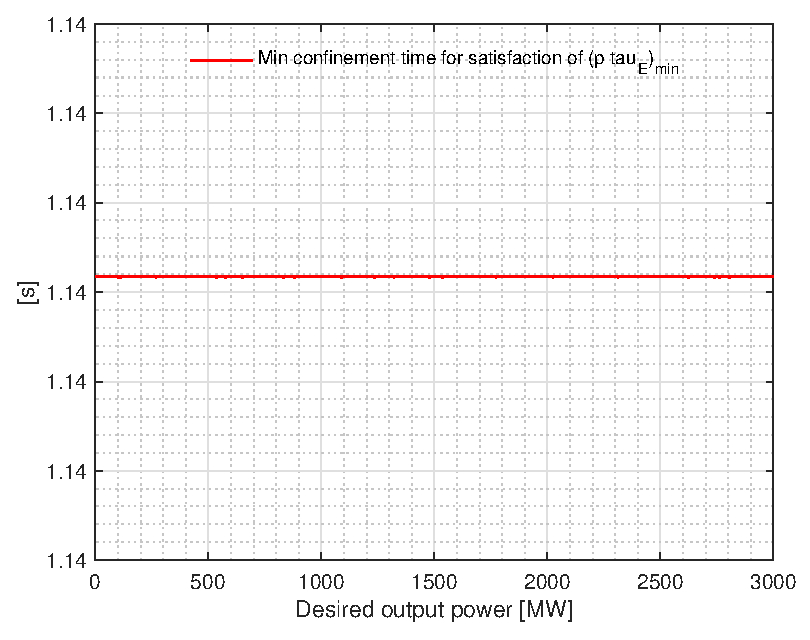
\includegraphics[width=\textwidth]{MatlabFigures/PE/f1.eps}
	\end{subfigure}
	~
	\begin{subfigure}[h!]{.45\textwidth}
		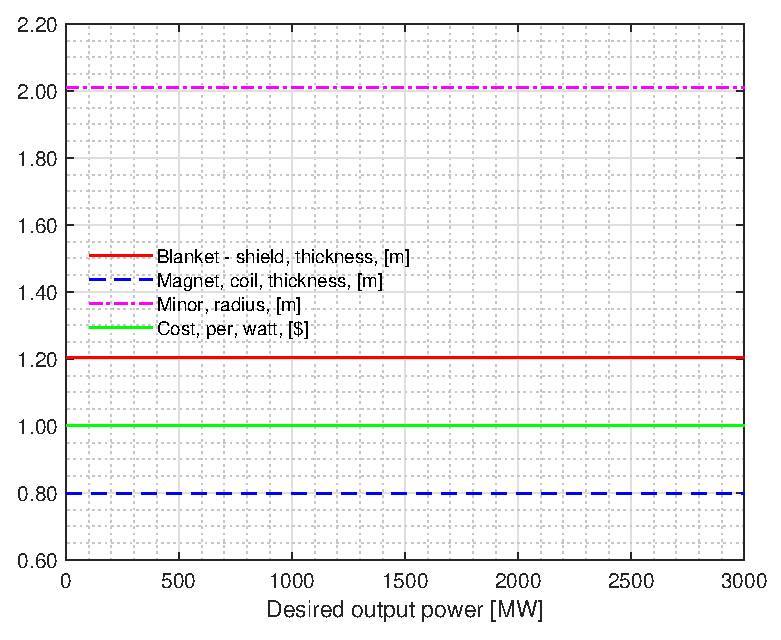
\includegraphics[width=\textwidth]{MatlabFigures/PE/f2.eps}
	\end{subfigure}

	\begin{subfigure}[h!]{.45\textwidth}
		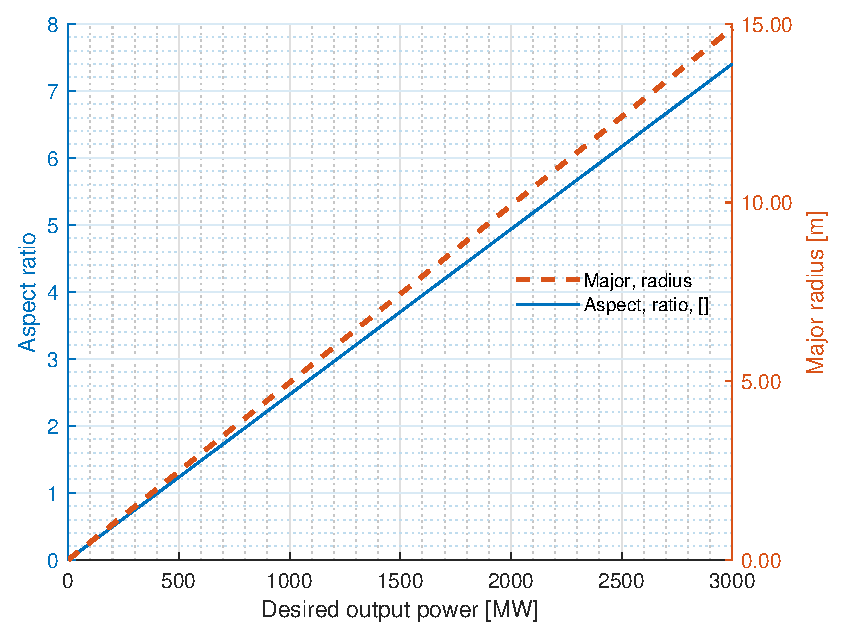
\includegraphics[width=\textwidth]{MatlabFigures/PE/f3.eps}
	\end{subfigure}
	~
	\begin{subfigure}[h!]{.45\textwidth}
		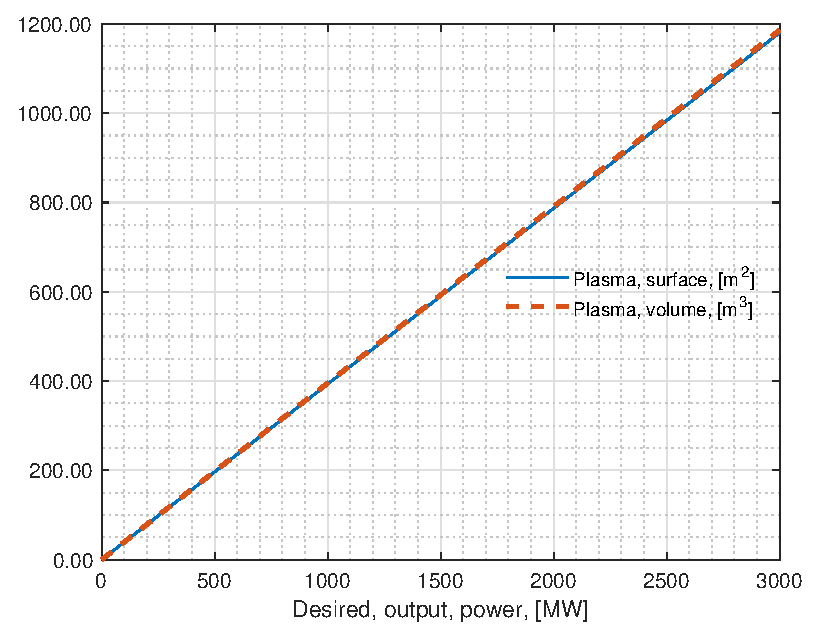
\includegraphics[width=\textwidth]{MatlabFigures/PE/f4.eps}
	\end{subfigure}

	\begin{subfigure}[h!]{.45\textwidth}
		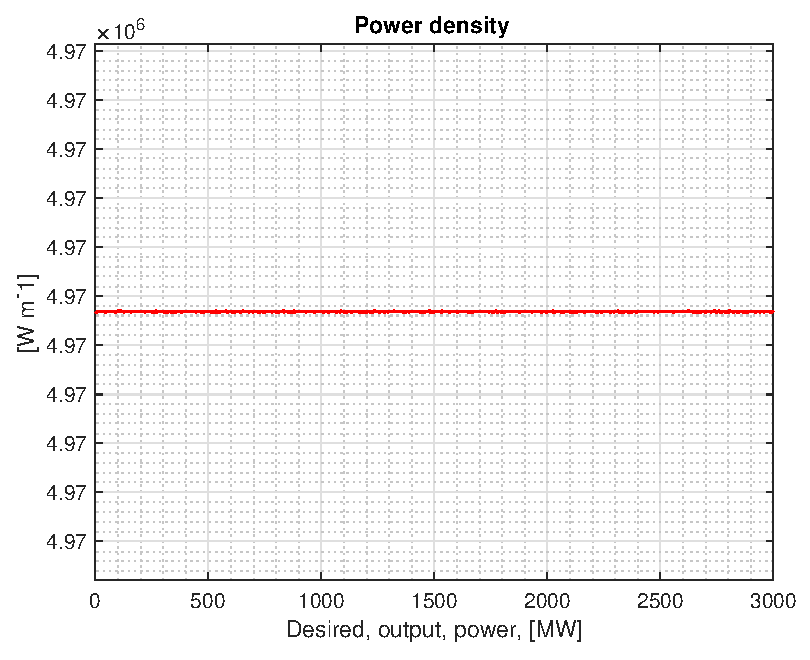
\includegraphics[width=\textwidth]{MatlabFigures/PE/f5.eps}
	\end{subfigure}
	~
	\begin{subfigure}[h!]{.45\textwidth}
		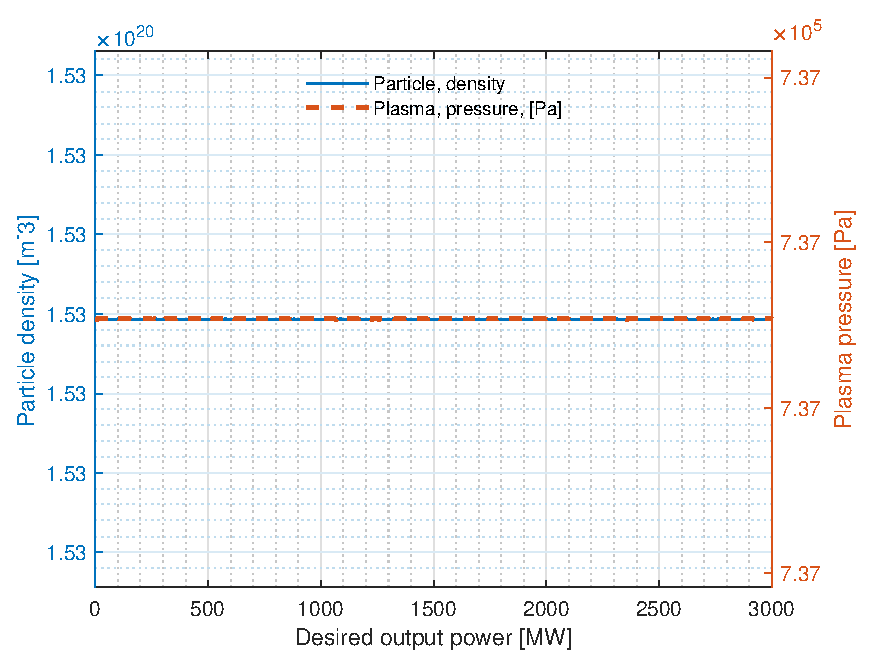
\includegraphics[width=\textwidth]{MatlabFigures/PE/f6.eps}
	\end{subfigure}

	\begin{subfigure}[h!]{.45\textwidth}
		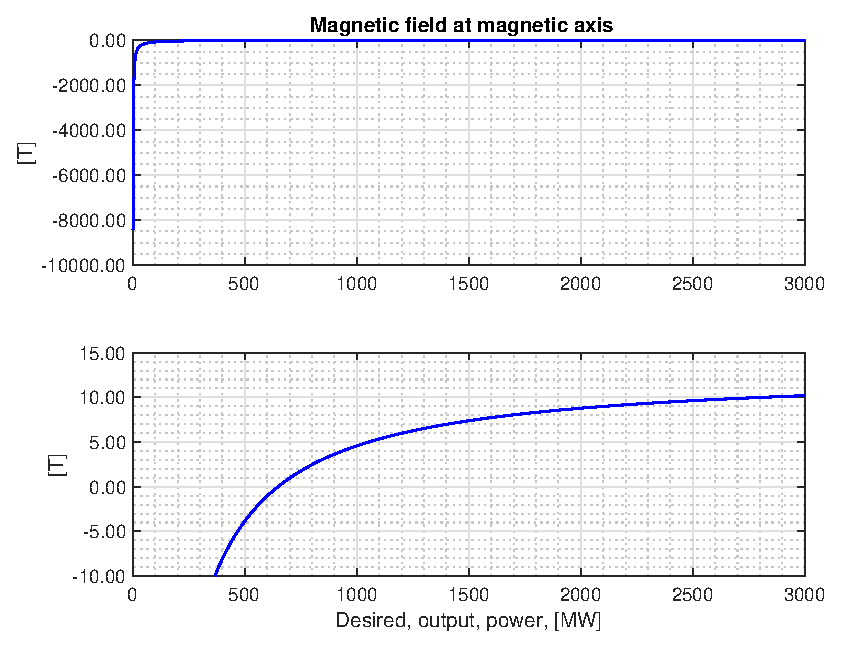
\includegraphics[width=\textwidth]{MatlabFigures/PE/f7.eps}
	\end{subfigure}
	~
	\begin{subfigure}[h!]{.45\textwidth}
		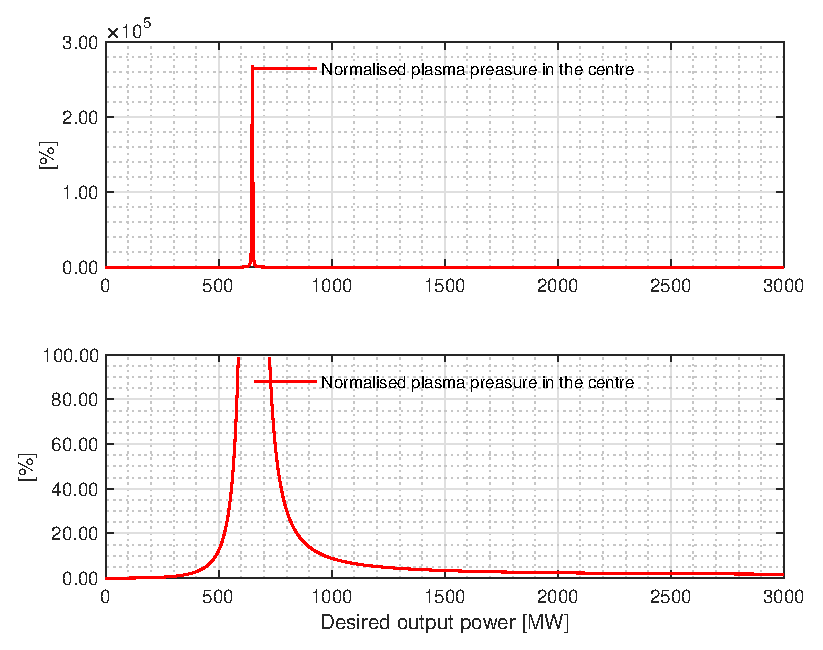
\includegraphics[width=\textwidth]{MatlabFigures/PE/f8.eps}
	\end{subfigure}
\end{figure}
\begin{figure}[H]
	\centering
	\begin{subfigure}[h!]{.45\textwidth}
		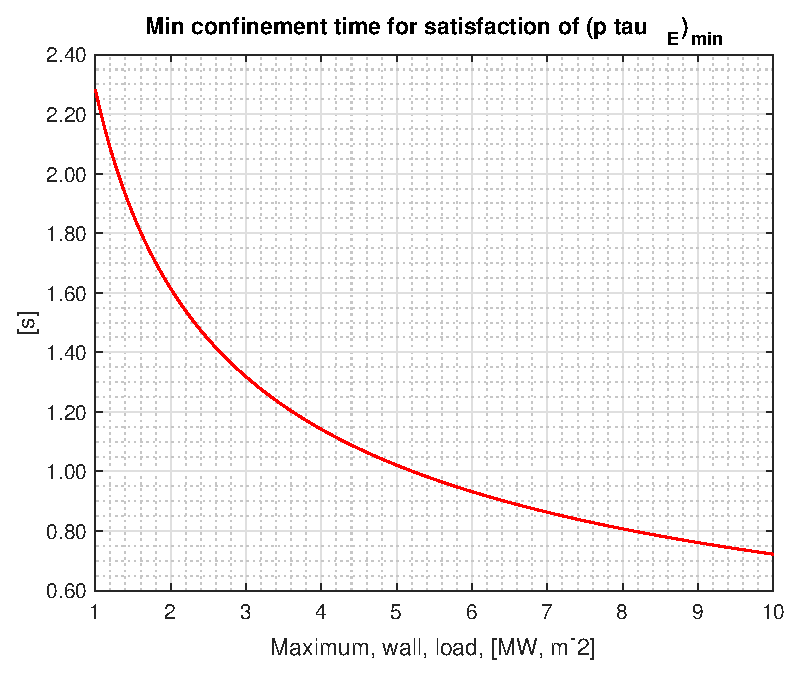
\includegraphics[width=\textwidth]{MatlabFigures/PW/f1.eps}
	\end{subfigure}
	~
	\begin{subfigure}[h!]{.45\textwidth}
		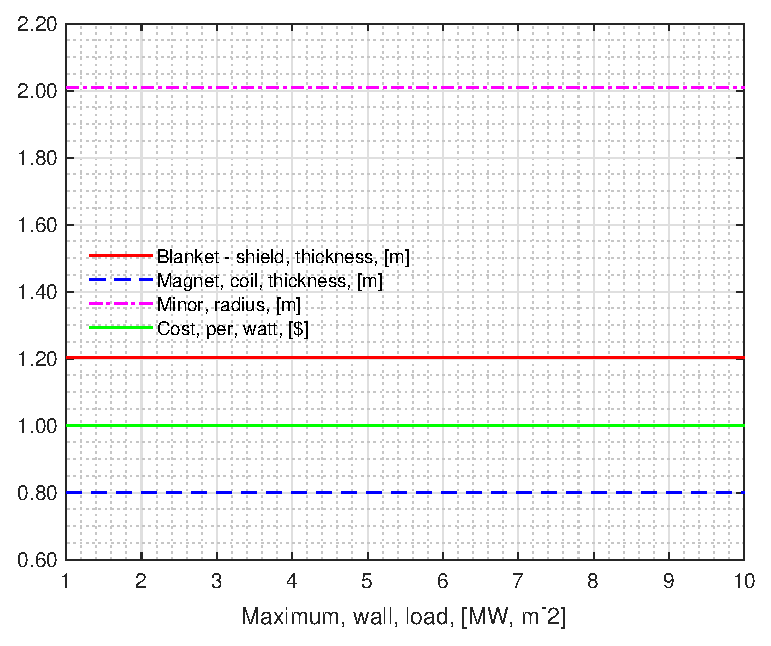
\includegraphics[width=\textwidth]{MatlabFigures/PW/f2.eps}
	\end{subfigure}

	\begin{subfigure}[h!]{.45\textwidth}
		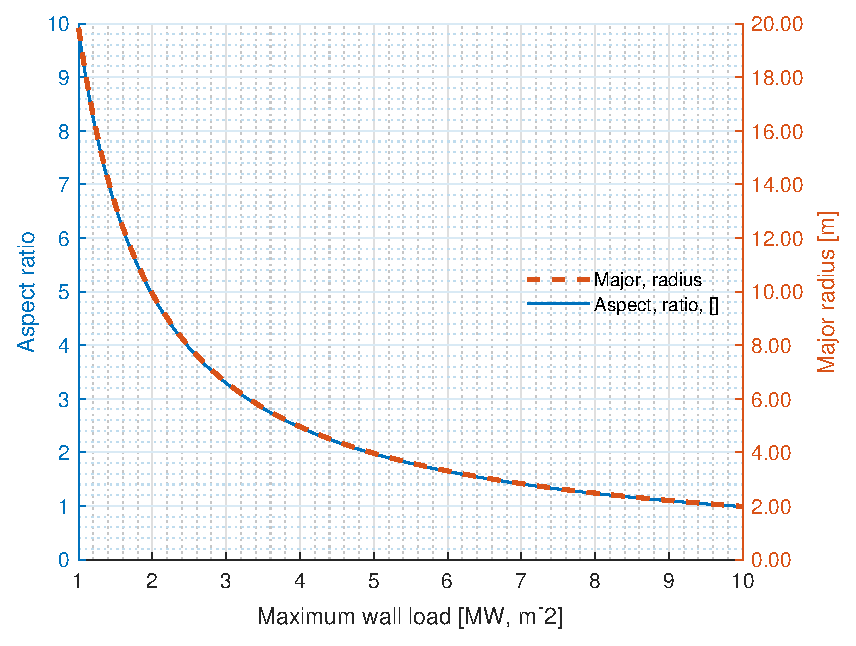
\includegraphics[width=\textwidth]{MatlabFigures/PW/f3.eps}
	\end{subfigure}
	~
	\begin{subfigure}[h!]{.45\textwidth}
		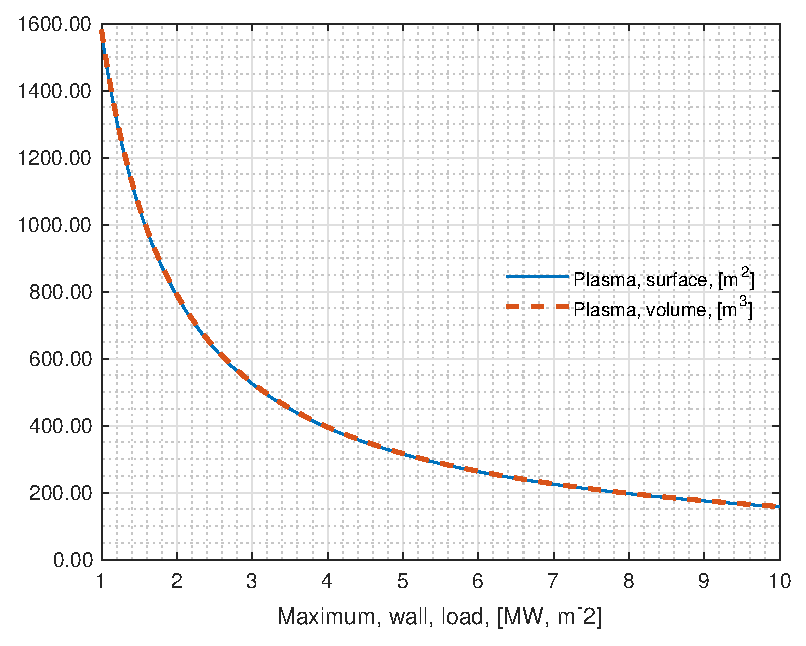
\includegraphics[width=\textwidth]{MatlabFigures/PW/f4.eps}
	\end{subfigure}

	\begin{subfigure}[h!]{.45\textwidth}
		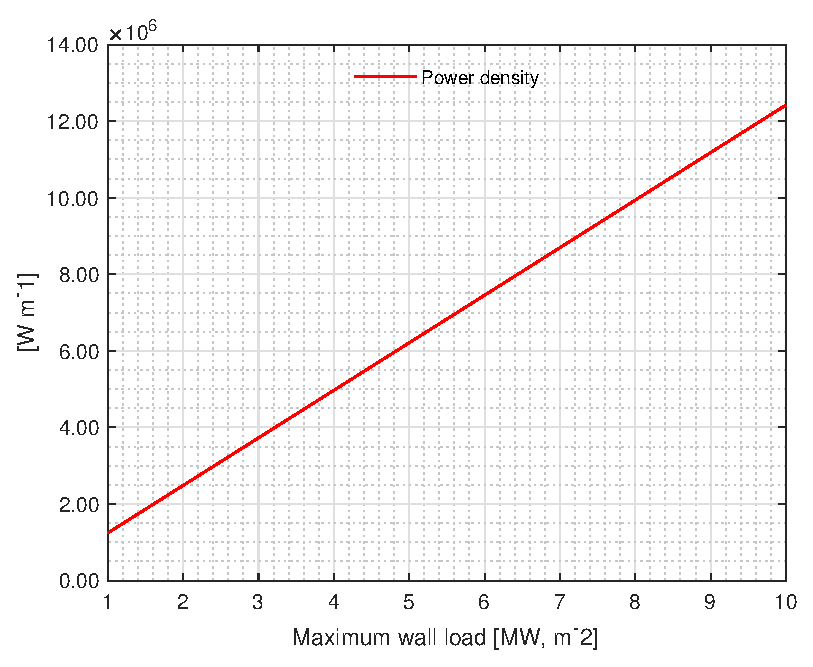
\includegraphics[width=\textwidth]{MatlabFigures/PW/f5.eps}
	\end{subfigure}
	~
	\begin{subfigure}[h!]{.45\textwidth}
		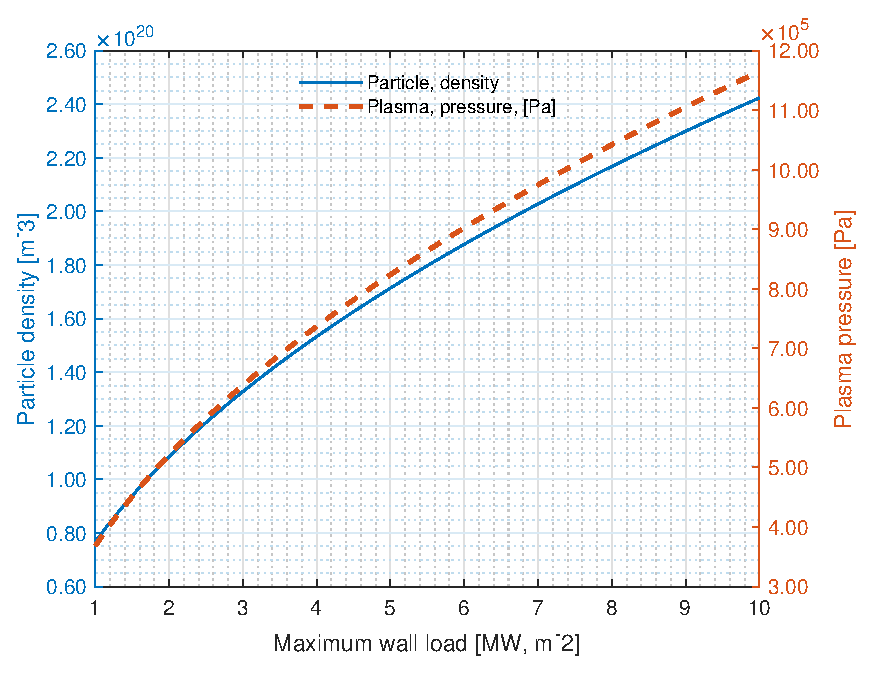
\includegraphics[width=\textwidth]{MatlabFigures/PW/f6.eps}
	\end{subfigure}

	\begin{subfigure}[h!]{.45\textwidth}
		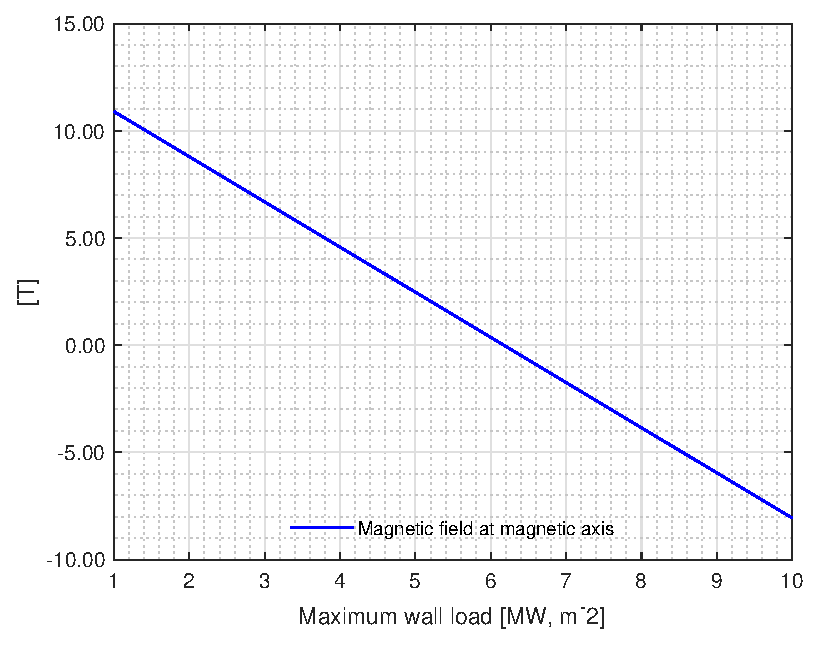
\includegraphics[width=\textwidth]{MatlabFigures/PW/f7.eps}
	\end{subfigure}
	~
	\begin{subfigure}[h!]{.45\textwidth}
		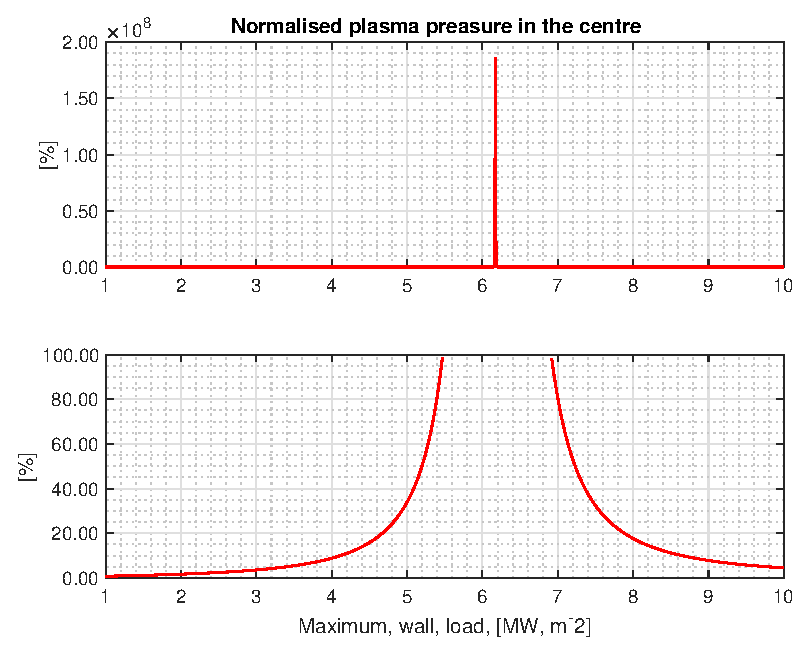
\includegraphics[width=\textwidth]{MatlabFigures/PW/f8.eps}
	\end{subfigure}
\end{figure}
\begin{figure}[H]
	\centering
	\begin{subfigure}[h!]{.45\textwidth}
		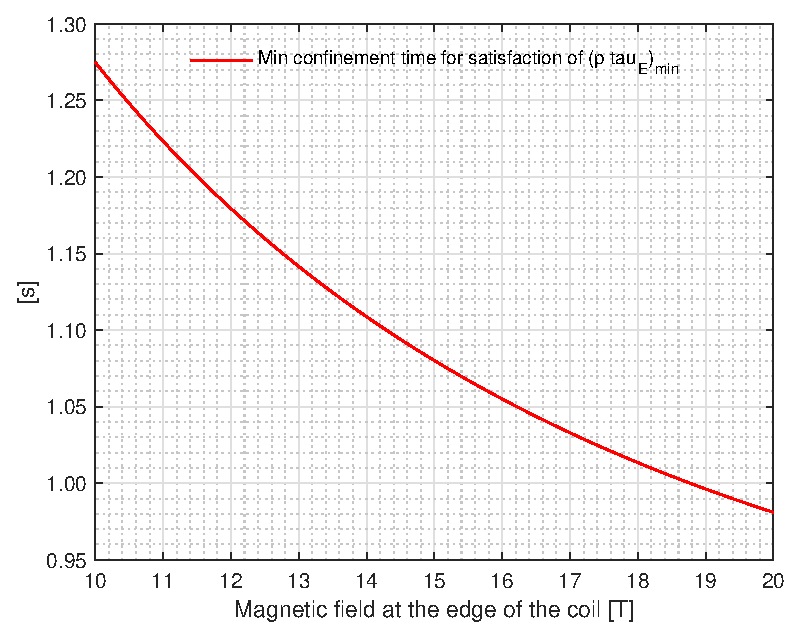
\includegraphics[width=\textwidth]{MatlabFigures/Bmax/f1.eps}
	\end{subfigure}
	~
	\begin{subfigure}[h!]{.45\textwidth}
		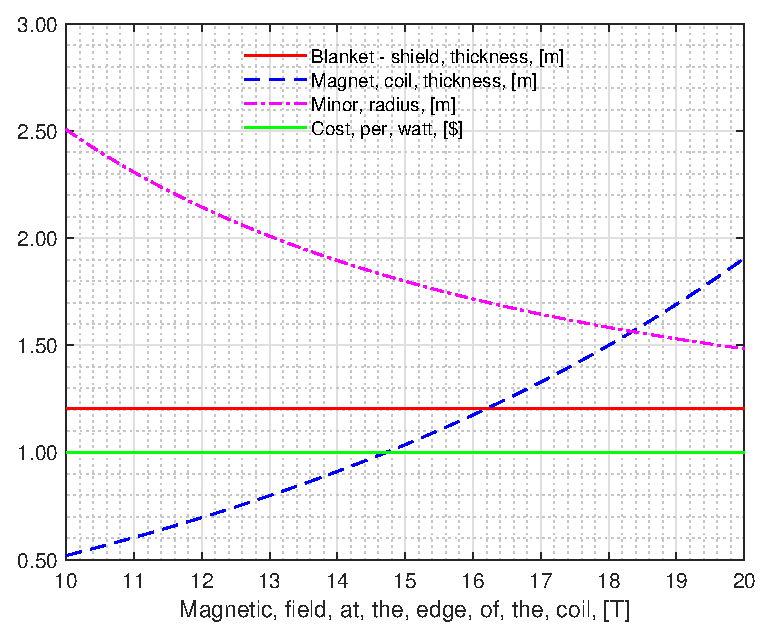
\includegraphics[width=\textwidth]{MatlabFigures/Bmax/f2.eps}
	\end{subfigure}

	\begin{subfigure}[h!]{.45\textwidth}
		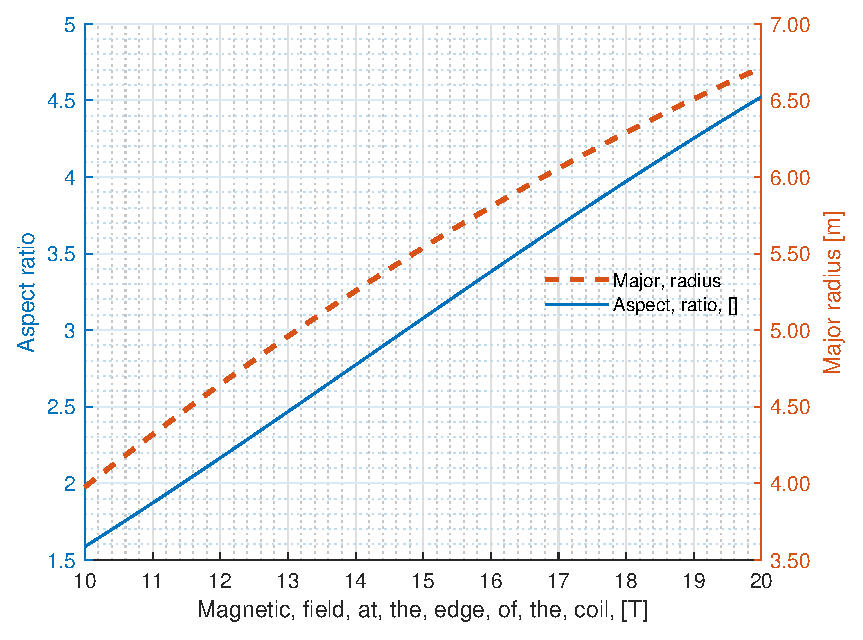
\includegraphics[width=\textwidth]{MatlabFigures/Bmax/f3.eps}
	\end{subfigure}
	~
	\begin{subfigure}[h!]{.45\textwidth}
		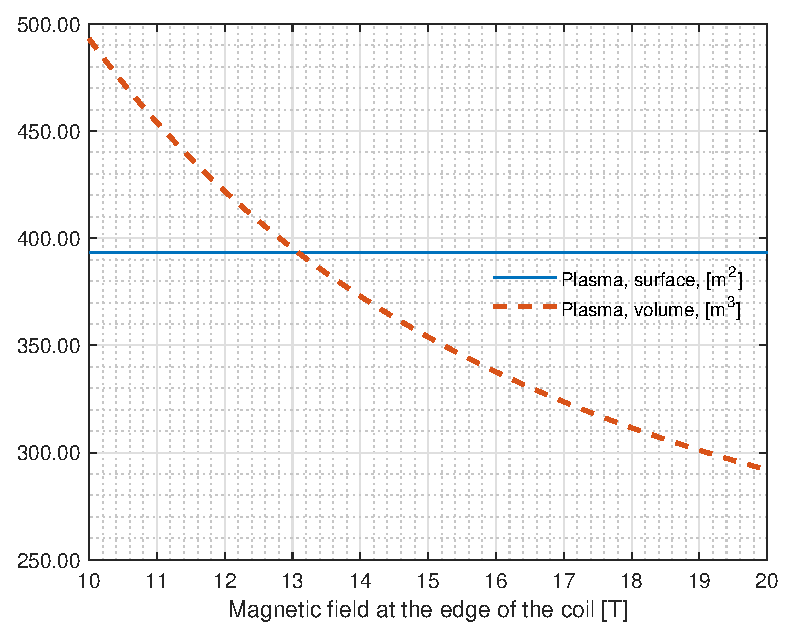
\includegraphics[width=\textwidth]{MatlabFigures/Bmax/f4.eps}
	\end{subfigure}

	\begin{subfigure}[h!]{.45\textwidth}
		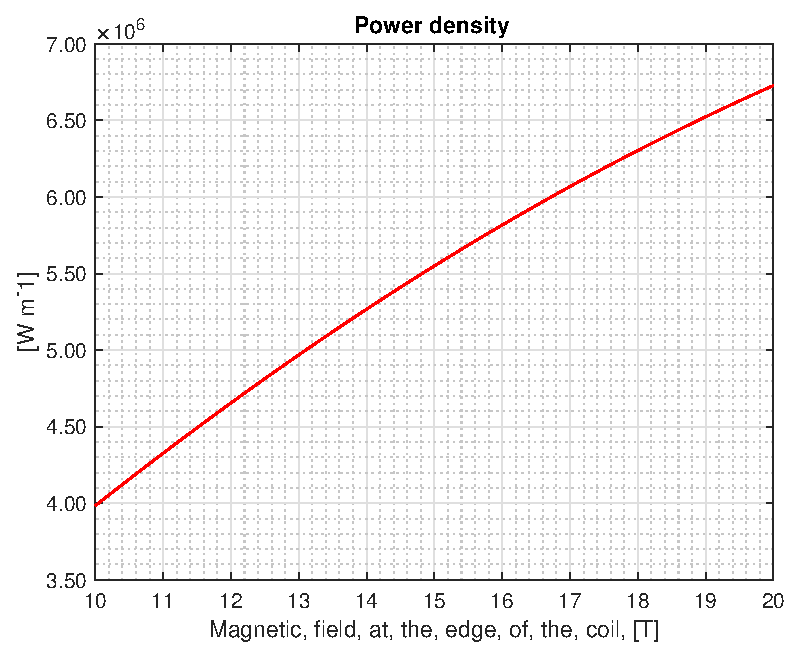
\includegraphics[width=\textwidth]{MatlabFigures/Bmax/f5.eps}
	\end{subfigure}
	~
	\begin{subfigure}[h!]{.45\textwidth}
		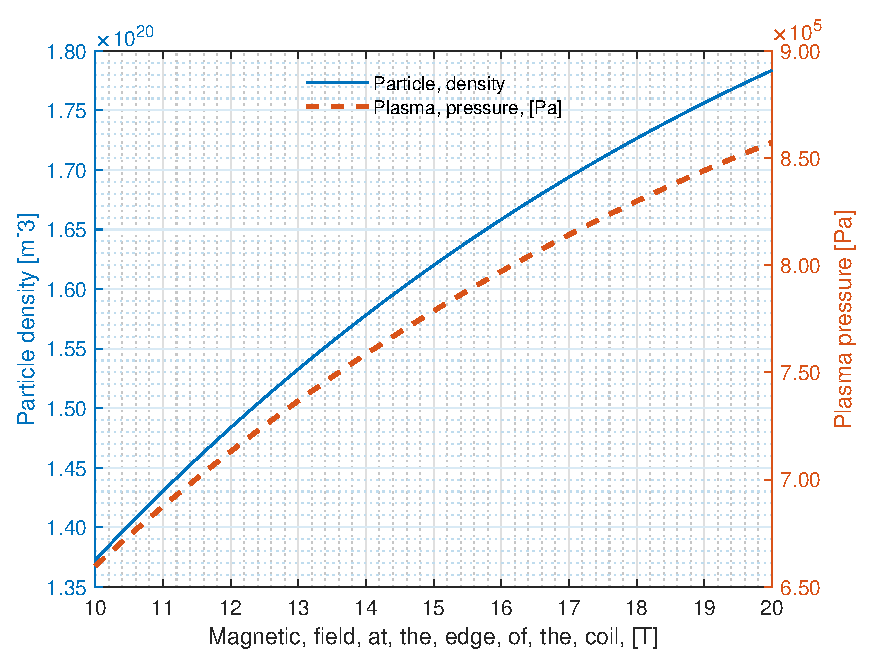
\includegraphics[width=\textwidth]{MatlabFigures/Bmax/f6.eps}
	\end{subfigure}

	\begin{subfigure}[h!]{.45\textwidth}
		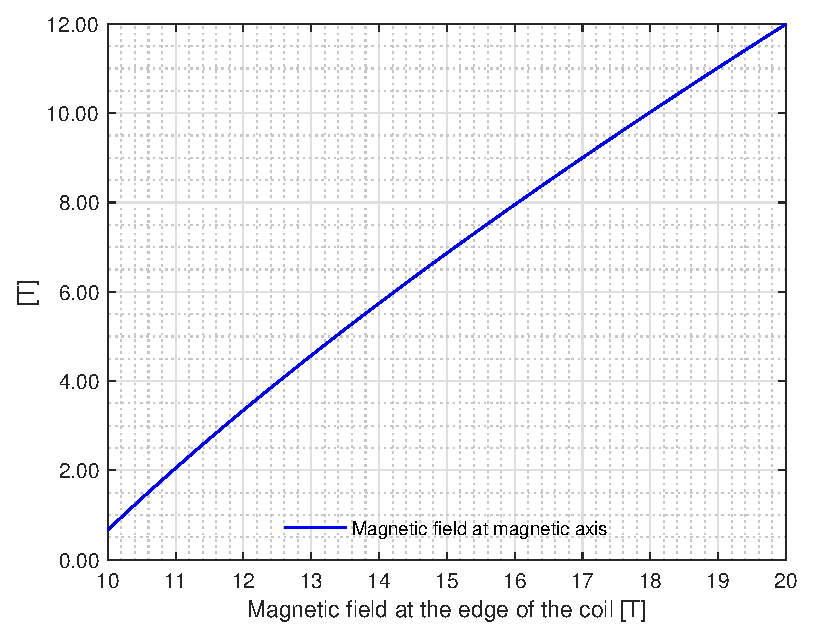
\includegraphics[width=\textwidth]{MatlabFigures/Bmax/f7.eps}
	\end{subfigure}
	~
	\begin{subfigure}[h!]{.45\textwidth}
		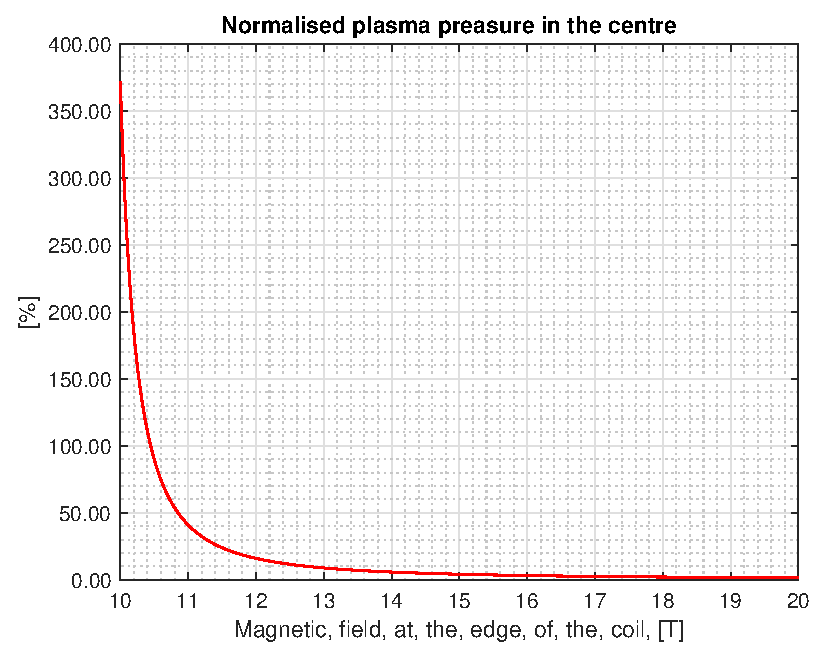
\includegraphics[width=\textwidth]{MatlabFigures/Bmax/f8.eps}
	\end{subfigure}
\end{figure}
\begin{figure}[H]
	\centering
	\begin{subfigure}[h!]{.45\textwidth}
		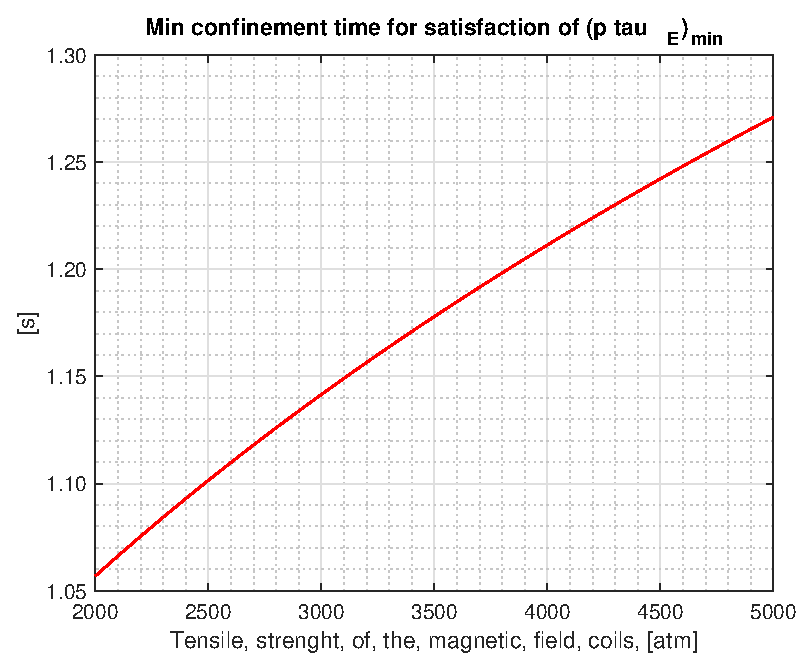
\includegraphics[width=\textwidth]{MatlabFigures/sigmamax/f1.eps}
	\end{subfigure}
	~
	\begin{subfigure}[h!]{.45\textwidth}
		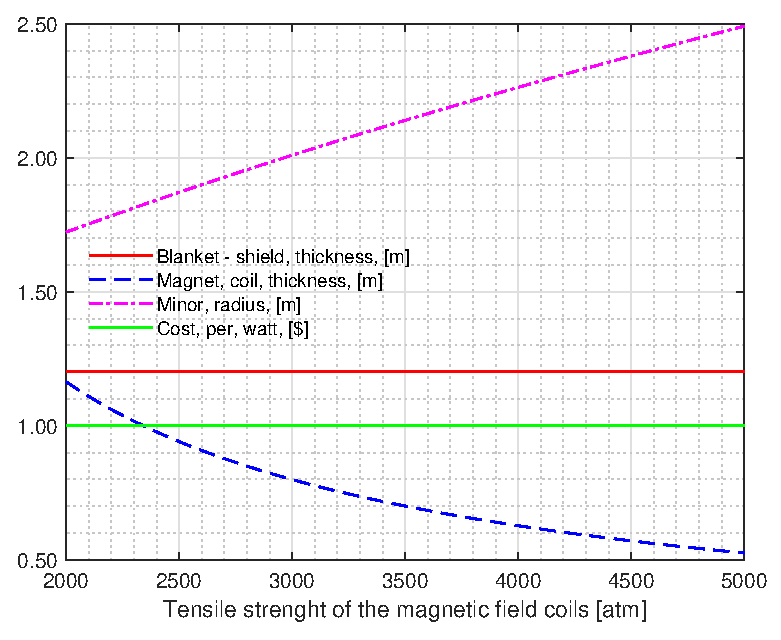
\includegraphics[width=\textwidth]{MatlabFigures/sigmamax/f2.eps}
	\end{subfigure}

	\begin{subfigure}[h!]{.45\textwidth}
		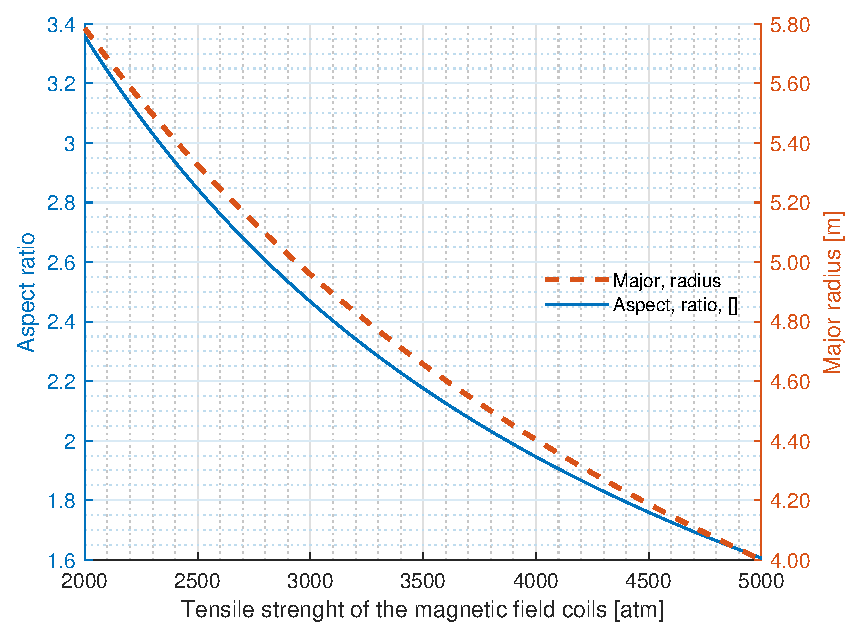
\includegraphics[width=\textwidth]{MatlabFigures/sigmamax/f3.eps}
	\end{subfigure}
	~
	\begin{subfigure}[h!]{.45\textwidth}
		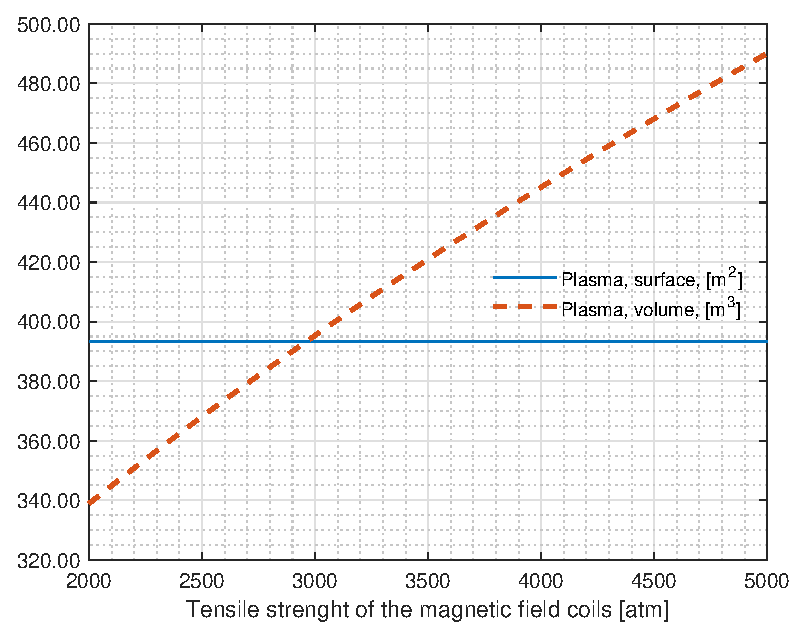
\includegraphics[width=\textwidth]{MatlabFigures/sigmamax/f4.eps}
	\end{subfigure}

	\begin{subfigure}[h!]{.45\textwidth}
		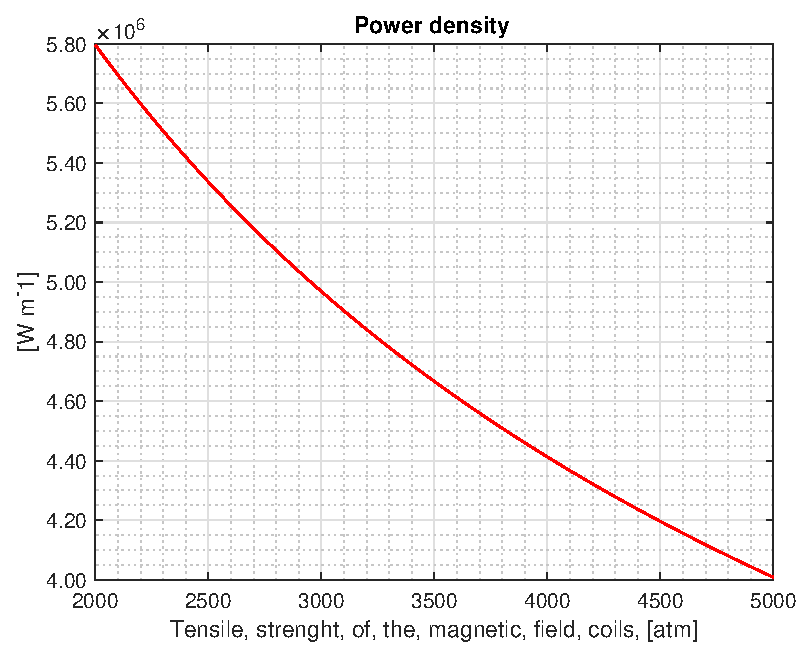
\includegraphics[width=\textwidth]{MatlabFigures/sigmamax/f5.eps}
	\end{subfigure}
	~
	\begin{subfigure}[h!]{.45\textwidth}
		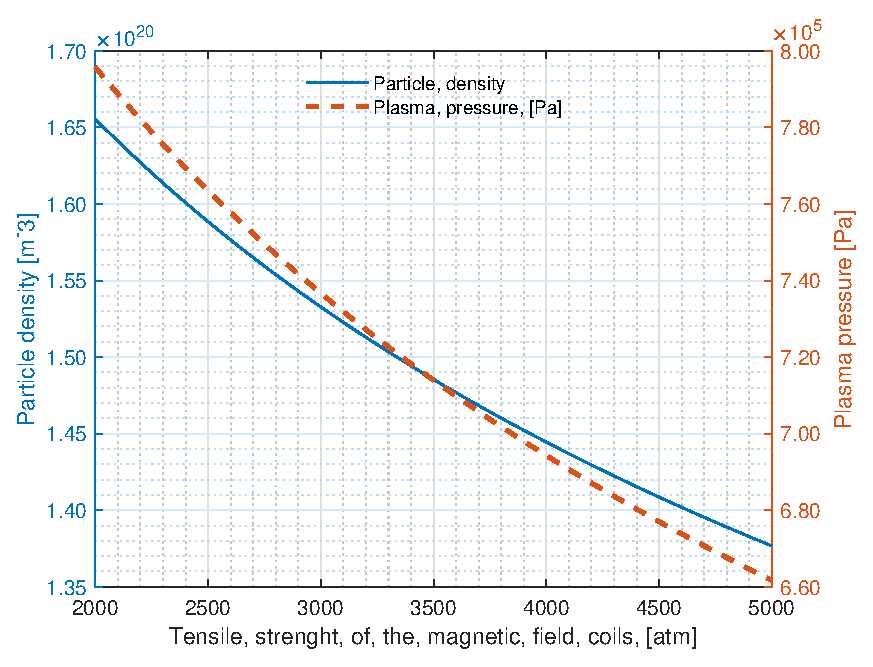
\includegraphics[width=\textwidth]{MatlabFigures/sigmamax/f6.eps}
	\end{subfigure}

	\begin{subfigure}[h!]{.45\textwidth}
		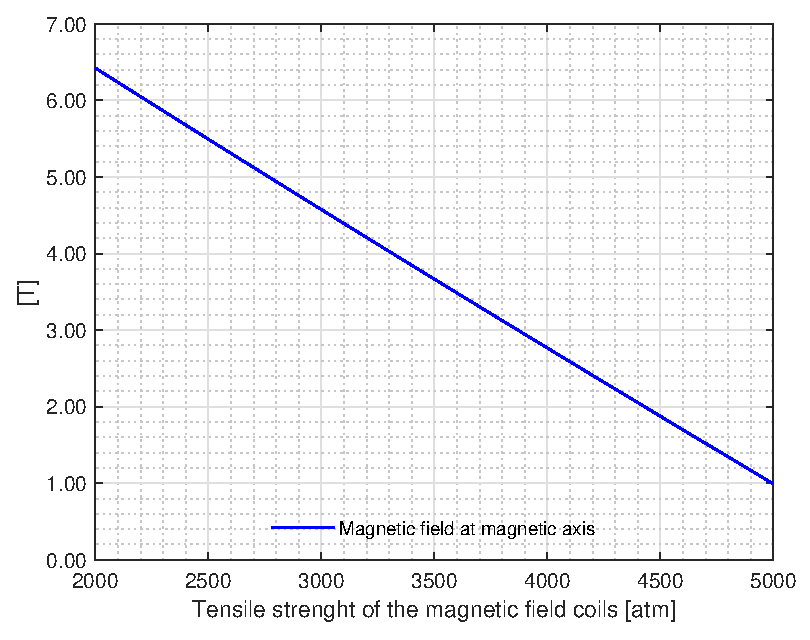
\includegraphics[width=\textwidth]{MatlabFigures/sigmamax/f7.eps}
	\end{subfigure}
	~
	\begin{subfigure}[h!]{.45\textwidth}
		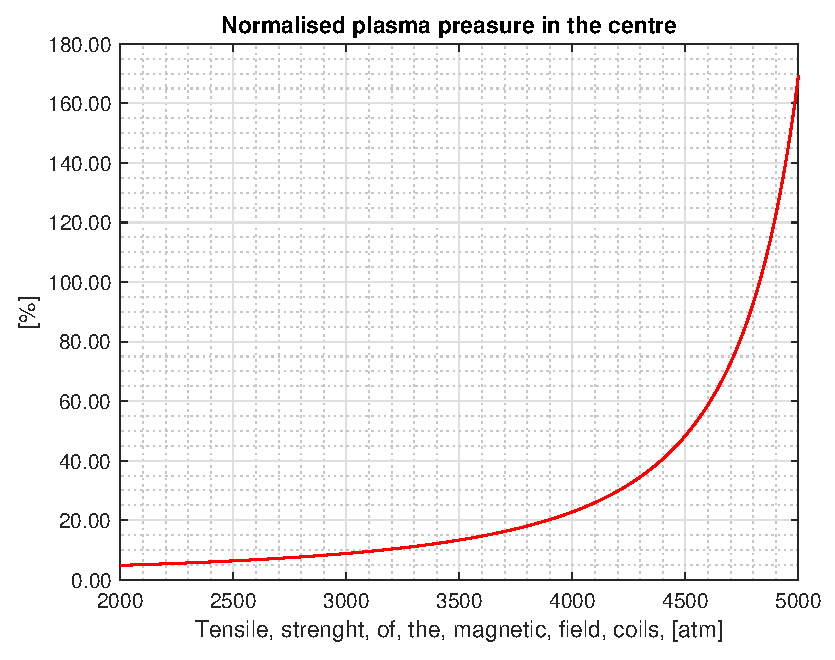
\includegraphics[width=\textwidth]{MatlabFigures/sigmamax/f8.eps}
	\end{subfigure}

\end{figure}
\newpage
\section{interferometer.m}\label{inter}
\inputminted[bgcolor=Black,linenos=true]{matlab}{Listings/interferometer.m}
\section{PhaseShiftDensity.m}
\inputminted[bgcolor=Black,linenos=true]{matlab}{Listings/PhaseShiftDensity.m}\label{PSD}

\end{document}
